\documentclass[11pt]{article}
\usepackage{myz310e-notes}
\usepackage{needspace}
\hypersetup{pdftitle={Optimisation: gradients, gradient descent and its stochastic variants},pdfauthor={Emre Onur Kahya},pdfsubject={MYZ 310E Machine Learning in Physics, Fall 2026, lecture note 7 (week 4)}}
\newcommand{\gvec}{\vect{g}}
\newcommand{\dvec}{\vect{\delta}}
\newcommand{\vvec}{\vect{v}}
\newcommand{\mvec}{\vect{m}}
\newcommand{\evec}{\vect{e}}
\newcommand{\errv}{\vect{\Delta}}
\newcommand{\uvec}{\vect{u}}
\newcommand{\qvec}{\vect{q}}

\begin{document}
\NoteTitle{7}{4}{Optimisation: gradients, gradient\\ descent and its stochastic variants}{Optimisation}{%
Training a model means minimising an objective over its parameters. This note reviews the calculus needed --- partial
derivatives, gradients, the Hessian --- and derives gradient descent from a Taylor expansion: why the negative gradient
is the steepest direction, why the learning rate must stay below $2/\lambda_{\max}$, and how conditioning sets the
speed. It then treats convex and non-convex landscapes, the mini-batch stochastic gradients that make training on
large datasets possible, and the refinements used in practice: momentum, Newton's method, Adam, line search and early
stopping. Every method comes with pseudocode, its cost per iteration, and a small example computed by hand.}

\section{Learning is optimisation}\label{sec:problem}

The training phase of most algorithms in this course solves
\[
  \theta^* = \argmin_{\theta \in \R^p} J(\theta), \qquad
  J(\theta) = \frac1n \sum_{i=1}^n L\big(f_\theta(\x_i), y_i\big) + \lambda\,\Omega(\theta),
\]
the regularised empirical risk of Note~4, Section~7, as a function of the $p$ parameters. Minimising the sum or the
mean is the same problem, because multiplying a function by the positive constant $1/n$ does not move its minima; the
mean keeps the scale of $J$, and hence a good learning rate, independent of $n$. Maximising a likelihood is the same
as minimising its negative logarithm, so maximum-likelihood fitting (Note~2, Section~6) also fits this mould. Picture $J$
as a landscape over parameter space: training means finding a low point. A note on letters: $\lambda$ without an
index is the regularisation strength (apart from the unknown of an eigenvalue equation $\det(H - \lambda I) = 0$), while $\lambda_i$, $\lambda_{\max}$ and $\lambda_{\min}$ are eigenvalues
of the Hessian (Section~\ref{sec:lr}).

The number of parameters ranges from $p = 2$ for a straight line $f(x) = wx + b$ through $p = d + 1$ for logistic
regression on $d$ features (a linear classifier with a smooth convex loss, Note~9, Section~4) to $p \approx 10^{11}$ for a large language model.

\paragraph{Symbols for running times} Throughout, $n$ is the number of training examples, $d$ the number of input
features, $p$ the number of parameters, $n'$ the mini-batch size and $T$ the number of iterations. We assume that the
loss of one example and its gradient cost $O(p)$ operations; this holds for linear models ($p = d + 1$, one inner
product) and, as the notes of week~5 on neural networks will show, for networks too, where one forward and backward
pass costs a few operations per parameter. Hence one evaluation of $J$ or of $\nabla J$ costs $O(np)$. An optimiser
changes only the training cost: prediction with the trained model costs what the model costs ($O(p)$ per query for the
models above), so the running-time boxes of this note list training time and memory.

\paragraph{When gradients are not available} Every method of this note needs continuous parameters and an objective
whose gradient (or at least a subgradient) can be computed cheaply. Discrete choices --- the $k$ of $k$ nearest
neighbours, a histogram bin width, the splits of a tree, most hyperparameters --- have no gradient; they are chosen by
grid or random search on validation data (Note~4, Section~7). A piecewise-constant loss such as the 0--1 error has a
gradient that is zero almost everywhere, so it is replaced by a smooth \emph{surrogate} such as the logistic or hinge
loss (Note~4, Section~2).

\section{Derivatives, gradients and curvature}\label{sec:calculus}

This section collects the calculus that every optimiser in the note relies on, using one small function as a
running example.

\subsection{Partial derivatives, the gradient and the Hessian}\label{sec:grad}

For one variable, the derivative $J'(\theta) = \lim_{\epsilon\to 0}\big(J(\theta + \epsilon) - J(\theta)\big)/\epsilon$ is
the slope of the graph at $\theta$. For $J : \R^p \to \R$ the same limit, taken along one coordinate axis, is the partial derivative
\[
  \frac{\partial J}{\partial\theta_k}(\theta) = \lim_{\epsilon\to 0} \frac{J(\theta + \epsilon\,\evec_k) - J(\theta)}{\epsilon}
\]
($\evec_k$ is the $k$-th unit vector) measures the sensitivity of $J$ to a change of $\theta_k$ alone, the other
parameters held fixed; for $p = 1$ it is the ordinary derivative. In practice one differentiates with respect to $\theta_k$ treating the others as constants.
The \emph{gradient} collects the partial derivatives,
\[
  \nabla J(\theta) = \Big( \frac{\partial J}{\partial\theta_1}(\theta), \dots, \frac{\partial J}{\partial\theta_p}(\theta) \Big)\T \in \R^p ,
\]
and the $p \times p$ matrix of second derivatives is the \emph{Hessian}, $H_{kl} = \partial^2 J / \partial\theta_k\partial\theta_l$.
For smooth $J$ the order of differentiation does not matter, so $H$ is symmetric and has real eigenvalues and orthogonal
eigenvectors. Moving from $\theta$ along a vector $\uvec$, every coordinate changes as $\theta_k + \epsilon u_k$, with
$d(\theta_k + \epsilon u_k)/d\epsilon = u_k$, so the chain rule gives the \emph{directional derivative}
\begin{equation}\label{eq:directional}
  \frac{d}{d\epsilon} J(\theta + \epsilon\,\uvec)\Big|_{\epsilon = 0} = \sum_k \frac{\partial J}{\partial\theta_k}\,u_k = \nabla J(\theta)\T\uvec .
\end{equation}
The formula holds for any vector $\uvec$; for a unit vector it is the slope of $J$ in that direction.

\begin{worked}{gradient and Hessian of a two-parameter function}
Take
\[
  J(\theta_1, \theta_2) = \tfrac14\theta_1^4 - \theta_1\theta_2 + \tfrac12\theta_2^2 ,
\]
a small landscape that we shall reuse throughout the note. Differentiating with respect to one variable at a time,
\[
  \frac{\partial J}{\partial\theta_1} = \theta_1^3 - \theta_2, \qquad
  \frac{\partial J}{\partial\theta_2} = -\theta_1 + \theta_2, \qquad
  H(\theta) = \begin{pmatrix} 3\theta_1^2 & -1 \\ -1 & 1 \end{pmatrix},
\]
where $H_{11} = \partial(\theta_1^3 - \theta_2)/\partial\theta_1 = 3\theta_1^2$, $H_{12} = \partial(\theta_1^3 - \theta_2)/\partial\theta_2 = -1$,
$H_{21} = \partial(-\theta_1 + \theta_2)/\partial\theta_1 = -1$ (equal to $H_{12}$, as it must be) and $H_{22} = 1$.
At $\theta = (2, 1)$:
\[
  J = 4 - 2 + \tfrac12 = 2.5, \qquad \nabla J = \begin{pmatrix} 8 - 1 \\ -2 + 1 \end{pmatrix} = \begin{pmatrix} 7 \\ -1 \end{pmatrix}, \qquad
  H = \begin{pmatrix} 12 & -1 \\ -1 & 1 \end{pmatrix}.
\]
The function rises steeply when $\theta_1$ increases and falls slowly when $\theta_2$ increases. The eigenvalues of
$H(2,1)$ are $0.91$ and $12.09$: the surface curves upwards in every direction there, much more strongly along
(roughly) the $\theta_1$ axis.
\end{worked}

\paragraph{Two gradients that recur} For a constant vector $\vect{b}$, $\vect{b}\T\theta = \sum_k b_k\theta_k$ has
$\partial/\partial\theta_k = b_k$, so $\nabla(\vect{b}\T\theta) = \vect{b}$. For a symmetric matrix $A$, the quadratic
form $\frac12\theta\T A\theta = \frac12\sum_{i,j}\theta_i A_{ij}\theta_j$ has
$\partial/\partial\theta_k = \frac12\big(\sum_j A_{kj}\theta_j + \sum_i \theta_i A_{ik}\big) = (A\theta)_k$, using
$A_{ik} = A_{ki}$; so $\nabla\big(\frac12\theta\T A\theta\big) = A\theta$, and its Hessian is $A$ itself.

\subsection{Taylor expansion and the direction of steepest descent}

Taylor's theorem summarises what the gradient and the Hessian mean: for a small step $\dvec$,
\begin{equation}\label{eq:taylor}
  J(\theta + \dvec) = J(\theta) + \nabla J(\theta)\T\dvec + \tfrac12 \dvec\T H(\theta)\,\dvec + O(\norm{\dvec}^3) .
\end{equation}
The gradient gives the best linear approximation of $J$ near $\theta$, the Hessian the best quadratic correction.

\paragraph{Derivation: the negative gradient is the steepest descent direction} Take a step of small length
$\epsilon$ in the direction of a unit vector $\uvec$, $\dvec = \epsilon\uvec$. Keeping the first-order term of
\eqref{eq:taylor},
\[
  J(\theta + \epsilon\uvec) - J(\theta) \approx \epsilon\, \nabla J(\theta)\T\uvec .
\]
Which unit vector makes this change as negative as possible? The Cauchy--Schwarz inequality states
$|\vect{a}\T\vect{b}| \le \norm{\vect{a}}\,\norm{\vect{b}}$, with equality exactly when $\vect{a}$ and $\vect{b}$ are
parallel. With $\norm{\uvec} = 1$ it gives
\[
  -\norm{\nabla J(\theta)} \;\le\; \nabla J(\theta)\T\uvec \;\le\; \norm{\nabla J(\theta)} ,
\]
and the lower bound is reached only for $\uvec = -\nabla J(\theta)/\norm{\nabla J(\theta)}$. Two conclusions
follow. (i) The direction of \emph{steepest descent} is $-\nabla J$; the gradient itself points uphill, in the
direction of steepest ascent. (ii) The steepest slope equals $\norm{\nabla J}$. In addition, \eqref{eq:directional}
gives (iii): along a contour line $J$ is constant, so $\nabla J\T\uvec = 0$ for a tangent $\uvec$, and the gradient is
perpendicular to the contour lines. These statements describe the slope at $\theta$ itself. A step of finite length
follows them only approximately, because the gradient changes as $\theta$ moves; that is why they are called
\emph{local}, and why a long step in the steepest-descent direction can even increase $J$ (Section~\ref{sec:gd}).

In the worked example, at $(2, 1)$ the steepest descent direction is $-(7, -1)/\sqrt{50} = (-0.990, 0.141)$, along
which $J$ falls at rate $\sqrt{50} = 7.07$; moving along $-\evec_1$ instead it falls at rate $7$, along $+\evec_2$ at
rate $1$.

\subsection{Stationary points and their classification}\label{sec:stationary}

\paragraph{Derivation: at a minimum the gradient vanishes} Suppose $\theta^*$ is a local minimum but
$\gvec = \nabla J(\theta^*) \ne \vect{0}$. Step a little against the gradient, $\dvec = -\epsilon\gvec$. By
\eqref{eq:taylor}, $J(\theta^* + \dvec) = J(\theta^*) - \epsilon\norm{\gvec}^2 + O(\epsilon^2)$, which is smaller than
$J(\theta^*)$ for small enough $\epsilon > 0$: a contradiction. Hence every local minimum (of a differentiable $J$ on
all of $\R^p$) satisfies the \emph{stationarity condition}
\[
  \nabla J(\theta^*) = \vect{0}, \qquad \text{i.e.}\quad \frac{\partial J}{\partial\theta_k}(\theta^*) = 0 \quad (k = 1, \dots, p).
\]
The condition is necessary, not sufficient: maxima and saddle points satisfy it too.

\paragraph{The second-order test} At a stationary point the linear term of \eqref{eq:taylor} vanishes and
$J(\theta^* + \dvec) - J(\theta^*) \approx \frac12\dvec\T H\dvec$. Writing $H = \sum_i \lambda_i \qvec_i\qvec_i\T$ with
orthonormal eigenvectors $\qvec_i$,
\[
  \tfrac12\dvec\T H\dvec = \tfrac12\sum_i \lambda_i\, (\qvec_i\T\dvec)^2 .
\]
If all $\lambda_i > 0$ ($H$ positive definite) every small step raises $J$: a local minimum. If all $\lambda_i < 0$ it is
a local maximum. If some are positive and some negative, $J$ rises along some directions and falls along others: a
\emph{saddle point}. Zero eigenvalues leave the test inconclusive. For $p = 2$ a quick rule uses
$\det H = \lambda_1\lambda_2$ and $\operatorname{tr} H = \lambda_1 + \lambda_2$: $\det H < 0$ means a saddle;
$\det H > 0$ with $\operatorname{tr} H > 0$ a minimum; $\det H > 0$ with $\operatorname{tr} H < 0$ a maximum.

\begin{worked}{finding and classifying the stationary points}
For $J = \frac14\theta_1^4 - \theta_1\theta_2 + \frac12\theta_2^2$, set both partial derivatives to zero. The second
gives $\theta_2 = \theta_1$; substituting into the first, $\theta_1^3 - \theta_1 = \theta_1(\theta_1 - 1)(\theta_1 + 1) = 0$.
There are three stationary points:
\begin{center}\small
\begin{tabular}{@{}lcccl@{}}
\toprule
point & $J$ & $H$ & $\det H$, $\operatorname{tr} H$ & type \\
\midrule
$(1, 1)$ and $(-1, -1)$ & $-\frac14$ & $\begin{pmatrix} 3 & -1 \\ -1 & 1 \end{pmatrix}$ & $2,\ 4$ & minima (eigenvalues $2 \pm \sqrt2 = 0.59,\ 3.41$) \\[2ex]
$(0, 0)$ & $0$ & $\begin{pmatrix} 0 & -1 \\ -1 & 1 \end{pmatrix}$ & $-1,\ 1$ & saddle (eigenvalues $-0.62,\ 1.62$) \\
\bottomrule
\end{tabular}
\end{center}
Figure~\ref{fig:quartic} shows the landscape. Along the diagonal $\theta_1 = \theta_2 = s$ we have
$J = \frac14 s^4 - \frac12 s^2$, which falls from the saddle towards both minima; along the anti-diagonal $J$ rises.
\end{worked}

\begin{figure}[tbp]
\centering
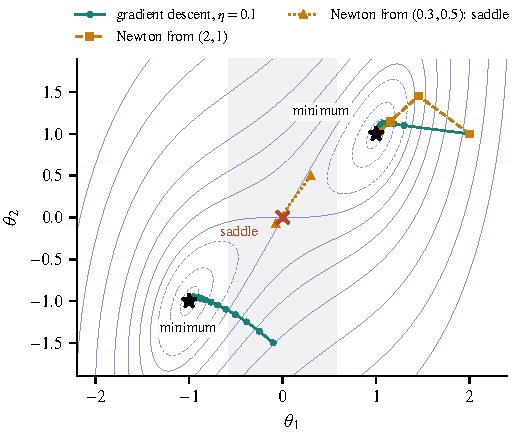
\includegraphics[width=0.52\linewidth]{figures/n7_quartic.pdf}
\caption{The landscape $J = \frac14\theta_1^4 - \theta_1\theta_2 + \frac12\theta_2^2$ with two minima (stars) and a
saddle (cross). In the shaded strip $|\theta_1| < 1/\sqrt3$ the Hessian is not positive definite, so $J$ is not convex
(Section~\ref{sec:convex}). Gradient descent with $\eta = 0.1$ from $(2, 1)$ and from $(-0.1, -1.5)$ reaches the
nearest minimum. Newton's method (Section~\ref{sec:newton}) from $(2, 1)$ reaches $(1, 1)$ in five steps to six
digits, but from $(0.3, 0.5)$ it converges to the saddle.}
\label{fig:quartic}
\end{figure}

\paragraph{Closed form or search} Sometimes $\nabla J = \vect{0}$ can be solved analytically, as in the example above.
In machine learning, the class means of the nearest-centroid classifier (which assigns a point to the class with the
closest mean, Note~9, Section~2), the maximum-likelihood Gaussian (Note~2, Section~6) and linear and ridge regression
(least squares, without or with a penalty $\lambda\norm{\vect{w}}^2$, Note~8) are such cases: their equations can be solved in
closed form (for the means and the regression weights they are even linear in the parameters). Usually they cannot be
solved, and we must search. Trying all
values on a grid (exhaustive search) costs $G^p$ evaluations of $J$ for $G$ values per parameter, each $O(np)$, so
$O(G^p\,np)$ in total. That is hopeless beyond a handful of parameters --- ten values per parameter and $p = 20$
already give $10^{20}$ evaluations, the curse of dimensionality of Note~3 once more --- so we follow the local slope
instead. Grid and random search remain the method of choice for a few hyperparameters (Note~4, Section~7).

\section{Gradient descent}\label{sec:gd}

Starting from an initial $\theta_0$ (random, or by a heuristic suited to the model), repeat
\begin{equation}\label{eq:gd}
  \theta_{t+1} = \theta_t - \eta\, \nabla J(\theta_t),
\end{equation}
where the \emph{learning rate} (step size) $\eta > 0$ is a hyperparameter. By Section~\ref{sec:calculus}, each step
moves in the locally steepest downhill direction, and for small enough $\eta$ it decreases $J$:
$J(\theta_{t+1}) \approx J(\theta_t) - \eta\norm{\nabla J(\theta_t)}^2$.

\paragraph{Notation for iterates} The subscript $t = 0, 1, 2, \dots$ on $\theta_t$ counts iterations. In the
two-parameter examples, where $\theta_1$ and $\theta_2$ already denote the two components of $\theta$, we write the
iterates with a superscript instead, $\theta^{(t)} = (\theta^{(t)}_1, \theta^{(t)}_2)$.

\subsection{The algorithm and its cost}

Algorithm~\ref{alg:gd} spells out batch gradient descent with the usual stopping rules: a small gradient norm, a
negligible relative change of $J$, or an exhausted iteration budget. Stopping when the parameters hardly change is the
gradient-norm test in disguise, since $\norm{\theta_{t+1} - \theta_t} = \eta\norm{\nabla J(\theta_t)}$ for a fixed $\eta$. One may also stop earlier, when the validation
error stops improving (early stopping, Section~\ref{sec:early}).

\begin{algorithm}[H]
\caption{Batch gradient descent with stopping rules}\label{alg:gd}
\begin{algorithmic}[1]
\Require objective $J$ and its gradient $\nabla J$; start $\theta_0$; learning rate $\eta$; tolerances $\epsilon_g, \epsilon_J$; maximum $T$
\Ensure approximate minimiser $\theta$
\Function{GradientDescent}{$\theta_0, \eta$}
  \State $\theta \gets \theta_0$, \quad $J_{\text{old}} \gets J(\theta)$
  \For{$t = 0, 1, \dots, T - 1$}
    \State $\gvec \gets \nabla J(\theta)$ \Comment{mean of $n$ per-example gradients: $O(np)$}
    \If{$\norm{\gvec} < \epsilon_g$} \Return $\theta$ \Comment{(nearly) stationary}\EndIf
    \State $\theta \gets \theta - \eta\,\gvec$ \Comment{$O(p)$; with constraints, $\Pi(\theta - \eta\gvec)$ (Section~\ref{sec:constraints})}
    \State $J_{\text{new}} \gets J(\theta)$ \Comment{monitoring: $O(np)$; if $J$ rises, reduce $\eta$}
    \If{$|J_{\text{old}} - J_{\text{new}}| < \epsilon_J\,(1 + |J_{\text{old}}|)$} \Return $\theta$ \EndIf
    \State $J_{\text{old}} \gets J_{\text{new}}$
  \EndFor
  \State \Return $\theta$ \Comment{iteration budget exhausted}
\EndFunction
\end{algorithmic}
\end{algorithm}

\begin{runtime}{batch gradient descent}
\textbf{Per iteration:} one full gradient, $O(np)$ ($O(nd)$ for a linear model: one pass over the data matrix), plus
$O(p)$ for the update. \textbf{Iterations:} on a quadratic with condition number $\kappa$ (Section~\ref{sec:lr}) and the
best fixed step, about $\frac{\kappa}{2}\ln(1/\tau)$ to reduce the error by a factor $\tau$ (twice that for
$\eta = 1/\lambda_{\max}$). \textbf{Memory:} $O(p)$ beyond the
$O(nd)$ data. \textbf{Prediction:} unchanged by the optimiser, $O(p)$ per query. \textbf{Hardware:} the gradient is a
matrix--vector product and vectorises well; the iterations themselves are sequential.
\end{runtime}

\begin{worked}{gradient descent in one dimension: stable, oscillating, diverging}
Let $J(\theta) = (\theta - 3)^2$, so $J'(\theta) = 2(\theta - 3)$, the minimum is $\theta^* = 3$ and the curvature is
$J'' = 2$. The update \eqref{eq:gd} reads
\[
  \theta_{t+1} - 3 = (\theta_t - 3) - 2\eta(\theta_t - 3) = (1 - 2\eta)(\theta_t - 3) ,
\]
so the distance to the minimum is multiplied by the same \emph{factor} $1 - 2\eta$ at every step. From $\theta_0 = 0$:
\begin{center}\small
\begin{tabular}{@{}lcccccccl@{}}
\toprule
$\eta$ & factor & $\theta_1$ & $\theta_2$ & $\theta_3$ & $\theta_4$ & $\theta_5$ & $J(\theta_5)$ & behaviour \\
\midrule
$0.1$  & $0.8$  & $0.6$ & $1.08$ & $1.464$ & $1.771$ & $2.017$ & $0.966$ & slow, monotone \\
$0.5$  & $0$    & $3$   & $3$    & $3$     & $3$     & $3$     & $0$     & exact in one step \\
$0.75$ & $-0.5$ & $4.5$ & $2.25$ & $3.375$ & $2.813$ & $3.094$ & $0.009$ & oscillates, converges \\
$1.1$  & $-1.2$ & $6.6$ & $-1.32$ & $8.184$ & $-3.221$ & $10.465$ & $55.7$ & oscillates, diverges \\
\bottomrule
\end{tabular}
\end{center}
Convergence requires $|1 - 2\eta| < 1$, i.e.\ $0 < \eta < 1 = 2/J''$. With a negative factor the iterate jumps across
the minimum at every step; whether the jumps shrink or grow depends on whether $|1 - 2\eta|$ is below or above one
(Figure~\ref{fig:steps1d}). The best step, $\eta = 1/J'' = 0.5$, lands on the minimum at once: it is the Newton step of
Section~\ref{sec:newton}.
\end{worked}

\begin{figure}[tbp]
\centering
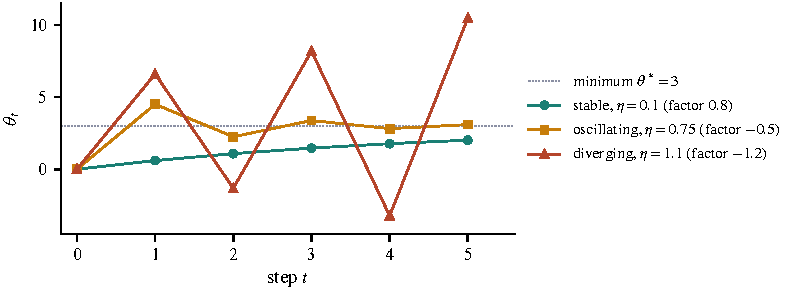
\includegraphics[width=0.68\linewidth]{figures/n7_steps_1d.pdf}
\caption{Iterates of gradient descent on $J(\theta) = (\theta - 3)^2$ from $\theta_0 = 0$ for three learning rates.
The distance to the minimum is multiplied by $1 - 2\eta$ at every step.}
\label{fig:steps1d}
\end{figure}

\subsection{What the learning rate does on a quadratic}\label{sec:lr}

Near a minimum, \eqref{eq:taylor} with $\dvec = \theta - \theta^*$ says that $J$ is approximately quadratic,
\[
  J(\theta) \approx J^* + \tfrac12 (\theta - \theta^*)\T A\, (\theta - \theta^*) ,
\]
with $J^* = J(\theta^*)$ and $A = H(\theta^*)$ symmetric and positive definite; the linear term has dropped out
because $\nabla J(\theta^*) = \vect{0}$. The behaviour of gradient descent on this model explains most
of what one sees in practice.

\paragraph{Derivation: the per-direction factor} Write $\errv = \theta - \theta^*$ for the error. By the quadratic-form
gradient of Section~\ref{sec:grad} (with $\errv$ in place of $\theta$), $\nabla J(\theta) = A\errv = A(\theta - \theta^*)$.
Substituting into \eqref{eq:gd},
\[
  \errv_{t+1} = \errv_t - \eta A\errv_t = (I - \eta A)\,\errv_t .
\]
Expand the error in the orthonormal eigenvectors of $A$, $\errv_t = \sum_i z_{i,t}\,\qvec_i$ with
$A\qvec_i = \lambda_i\qvec_i$ and coordinates $z_{i,t} = \qvec_i\T\errv_t$ (here $\lambda_i$ are eigenvalues, not the regularisation strength $\lambda$ of
Section~\ref{sec:problem}). Because $(I - \eta A)\qvec_i = (1 - \eta\lambda_i)\qvec_i$, the coordinates decouple:
\[
  z_{i,t+1} = (1 - \eta\lambda_i)\, z_{i,t}, \qquad\text{so}\qquad z_{i,t} = (1 - \eta\lambda_i)^t\, z_{i,0} .
\]
Along each eigenvector, gradient descent is exactly the one-dimensional example above, with curvature $\lambda_i$.

\paragraph{Derivation: the convergence condition} The error tends to zero from every start if and only if
$|1 - \eta\lambda_i| < 1$ for all $i$, i.e.\ $0 < \eta\lambda_i < 2$. The most curved direction is the binding one:
\begin{equation}\label{eq:stability}
  \eta < \frac{2}{\lambda_{\max}} .
\end{equation}
Per direction, $0 < \eta\lambda_i < 1$ gives a monotone approach, $\eta\lambda_i = 1$ one-step convergence,
$1 < \eta\lambda_i < 2$ a damped oscillation across the valley and $\eta\lambda_i > 2$ an oscillation with growing
amplitude.

\paragraph{Derivation: the best fixed step and the condition number} The slowest direction determines the overall
speed. Because the $\qvec_i$ are orthonormal, $\norm{\errv_t}^2 = \sum_i z_{i,t}^2$, and each $z_i$ is multiplied by
$|1 - \eta\lambda_i| \le \rho(\eta)$, where
$\rho(\eta) = \max_i |1 - \eta\lambda_i| = \max(|1 - \eta\lambda_{\min}|,\, |1 - \eta\lambda_{\max}|)$. Hence
$\norm{\errv_{t+1}} \le \rho(\eta)\,\norm{\errv_t}$: the error norm is \emph{multiplied} by at most $\rho$ per step. The
first term decreases with $\eta$, the second increases once
$\eta > 1/\lambda_{\max}$, so the best $\eta$ balances them: $1 - \eta\lambda_{\min} = \eta\lambda_{\max} - 1$, giving
\[
  \eta_{\text{best}} = \frac{2}{\lambda_{\min} + \lambda_{\max}}, \qquad
  \rho_{\text{best}} = \frac{\lambda_{\max} - \lambda_{\min}}{\lambda_{\max} + \lambda_{\min}} = \frac{\kappa - 1}{\kappa + 1},
  \qquad \kappa = \frac{\lambda_{\max}}{\lambda_{\min}} ,
\]
where $\kappa$ is the \emph{condition number}. ``Reducing the error by a factor $\tau$'' means multiplying it by
$\tau < 1$. After $t$ steps the error is at most $\rho^t$ times its start, so $\rho^t = \tau$ needs
$t = \ln(1/\tau)/\ln(1/\rho)$ steps. Writing $\rho_{\text{best}} = (1 - 1/\kappa)/(1 + 1/\kappa)$ and using
$\ln(1 + x) \approx x$ for small $x$, $\ln(1/\rho_{\text{best}}) = \ln(1 + 1/\kappa) - \ln(1 - 1/\kappa) \approx 2/\kappa$
for large $\kappa$, so about $\frac{\kappa}{2}\ln(1/\tau)$ steps are needed: elongated valleys are hard. For an error reduction of $10^{-6}$ this is 62 steps for $\kappa = 9$, 173 for $\kappa = 25$, 691 for
$\kappa = 100$ and 69\,078 for $\kappa = 10^4$. Only the ratio $\kappa$ matters, not the size of the eigenvalues:
multiplying $J$ by a constant multiplies every $\lambda_i$ by it, the best $\eta$ changes by the inverse factor, and
$\rho_{\text{best}}$, which depends only on $\kappa$, is unchanged.

\begin{worked}{gradient descent on a two-dimensional quadratic}
Let $J(\theta) = \frac12\theta\T A\theta$ with $A = \begin{pmatrix} 5 & 4 \\ 4 & 5\end{pmatrix}$, i.e.\
$J = \frac12(5\theta_1^2 + 8\theta_1\theta_2 + 5\theta_2^2)$, with minimum $\theta^* = \vect{0}$ and
$\nabla J = (5\theta_1 + 4\theta_2,\ 4\theta_1 + 5\theta_2)$. From $\det(A - \lambda I) = (5 - \lambda)^2 - 16 = 0$ the
eigenvalues are $\lambda_{\max} = 9$ with eigenvector along $(1, 1)$ and $\lambda_{\min} = 1$ along $(1, -1)$: $\kappa = 9$, the
stability limit is $\eta < 2/9 = 0.222$ and the best fixed step is $\eta = 2/(1 + 9) = 0.2$ with $\rho = 0.8$.

Start at $\theta^{(0)} = (3, 1) = 2\,(1, 1) + 1\,(1, -1)$, where $J = 37$ and $\nabla J = (19, 17)$. With $\eta = 0.1$ the
first step is $\theta^{(1)} = (3, 1) - 0.1\,(19, 17) = (1.1, -0.7)$. The eigen-decomposition predicts the same thing at a
glance: the $(1, 1)$ part is multiplied by $1 - 0.1 \cdot 9 = 0.1$ and the $(1, -1)$ part by $1 - 0.1 \cdot 1 = 0.9$,
so $\theta^{(t)} = 2\,(0.1)^t(1, 1) + (0.9)^t(1, -1)$. For three step sizes:
\begin{center}\small
\begin{tabular}{@{}lccccc@{}}
\toprule
$\eta$ & factors $(1, 1)$, $(1, -1)$ & $\theta^{(1)}$ & $\theta^{(2)}$ & $\theta^{(3)}$ & $J(\theta^{(1)}), J(\theta^{(2)}), J(\theta^{(3)})$ \\
\midrule
$0.1$  & $0.1,\ 0.9$   & $(1.1, -0.7)$   & $(0.83, -0.79)$  & $(0.731, -0.727)$ & $1.17,\ 0.660,\ 0.531$ \\
$0.2$  & $-0.8,\ 0.8$  & $(-0.8, -2.4)$  & $(1.92, 0.64)$   & $(-0.512, -1.536)$ & $23.7,\ 15.2,\ 9.70$ \\
$0.25$ & $-1.25,\ 0.75$ & $(-1.75, -3.25)$ & $(3.69, 2.56)$ & $(-3.48, -4.33)$ & $56.8,\ 88.2,\ 137.5$ \\
\bottomrule
\end{tabular}
\end{center}
With $\eta = 0.1$ the steep direction is removed almost at once, but the shallow one shrinks only by $0.9$ per step.
With $\eta = 0.2$ the iterate jumps across the valley at every step (factor $-0.8$) and $J$ looks worse at first;
yet both directions now shrink by $0.8$, and after 40 steps $J = 6.5 \times 10^{-7}$ against $2.2 \times 10^{-4}$ for
$\eta = 0.1$. With $\eta = 0.25 > 2/9$ the steep direction grows by $1.25$ per step and the iteration diverges.
\end{worked}

Figure~\ref{fig:gdpaths} shows a valley with $\kappa = 25$. With $\eta = 0.01$ the descent is stable but crawls; with
$\eta = 0.075$, close to the limit $2/25 = 0.08$, it zigzags across the valley and makes steady progress.

\begin{figure}[tbp]
\centering
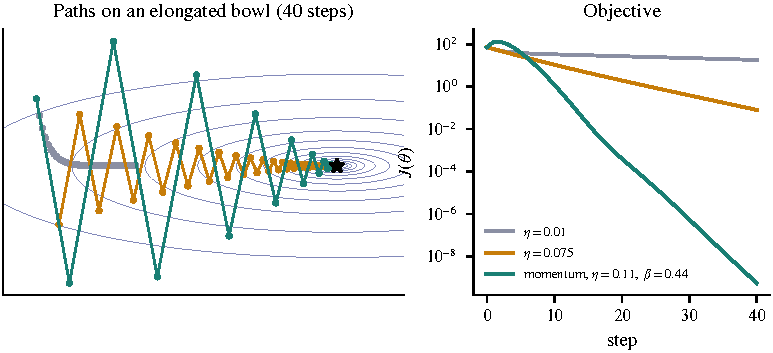
\includegraphics[width=0.88\linewidth]{figures/gd_paths.pdf}
\caption{Forty steps on $J(\theta) = \frac12(\theta_1^2 + 25\,\theta_2^2)$ ($\kappa = 25$) from the same start
$(-9, 1.6)$. Left:
horizontal axis $\theta_1$, vertical axis $\theta_2$ (the steep direction); the star is the minimum. After 40 steps
$J = 18$ for $\eta = 0.01$, $0.08$ for $\eta = 0.075$, and $5 \times 10^{-10}$ with momentum (Section~\ref{sec:momentum})
using Polyak's choice for $\kappa = 25$, $\eta = 4/36 = 0.11$ and $\beta = (4/6)^2 = 0.44$.}
\label{fig:gdpaths}
\end{figure}

\paragraph{Why features are standardised} The curvatures $\lambda_i$ come from the data. For the line fit
$J(w, b) = \frac1n\sum_i\frac12(wx_i + b - y_i)^2$ the first derivatives are $\frac1n\sum_i r_ix_i$ and
$\frac1n\sum_i r_i$ with residuals $r_i = wx_i + b - y_i$; differentiating once more ($\partial r_i/\partial w = x_i$,
$\partial r_i/\partial b = 1$) gives the Hessian as the matrix of averages
$\begin{pmatrix} \overline{x^2} & \bar x \\ \bar x & 1\end{pmatrix}$. With inputs $x = 1, 2, 3, 4$ it is
$\begin{pmatrix} 7.5 & 2.5 \\ 2.5 & 1\end{pmatrix}$, with eigenvalues $8.35$ and $0.150$ and $\kappa = 56$; after
centring the inputs ($x - 2.5$) it becomes $\operatorname{diag}(1.25, 1)$ with $\kappa = 1.25$. Very different
feature scales, or features far from zero mean, stretch the valley; standardising them (Note~5, Section~5) is often the
cheapest way to speed up gradient descent.

\subsection{Learning-rate schedules}\label{sec:schedules}

A fixed step is rarely ideal: large steps make fast early progress, small steps settle into the minimum, and with
stochastic gradients (Section~\ref{sec:sgd}) a decreasing step is needed to converge at all. Three common schedules,
all with peak value $\eta_{\max}$:
\begin{itemize}
\item $1/t$ decay: $\eta_t = \eta_{\max}\, t_0/(t_0 + t)$, halving after $t_0$ steps;
\item step decay: multiply $\eta$ by $0.1$ every fixed number of steps (or when the validation loss stalls);
\item linear warm-up over the first $W$ steps, then cosine decay up to step $T$: $\eta_t = \eta_{\max}\,(t + 1)/W$ for $t < W$, then
$\eta_t = \frac12\eta_{\max}\big(1 + \cos(\pi\,(t - W)/(T - W))\big)$ for $W \le t \le T$~\cite{loshchilov2017}.
\end{itemize}
The linear \emph{warm-up} from a small value avoids instabilities while the parameters are still random and the
curvature is unknown; the half-cosine decays slowly at first and approaches zero smoothly at the end (some recipes stop
the decay at a floor such as $0.1\,\eta_{\max}$).

\begin{worked}{three schedules side by side}
With $\eta_{\max} = 0.1$, $T = 1000$, $t_0 = 100$, step decay every 400 steps and a warm-up of $W = 100$ steps:
\begin{center}\small
\begin{tabular}{@{}lccccccc@{}}
\toprule
step $t$ & 0 & 50 & 100 & 325 & 550 & 775 & 1000 \\
\midrule
$1/t$ decay & 0.1000 & 0.0667 & 0.0500 & 0.0235 & 0.0154 & 0.0114 & 0.0091 \\
step decay  & 0.1 & 0.1 & 0.1 & 0.1 & 0.01 & 0.01 & 0.001 \\
warm-up + cosine & 0.0010 & 0.0510 & 0.1000 & 0.0854 & 0.0500 & 0.0146 & 0 \\
\bottomrule
\end{tabular}
\end{center}
For instance at $t = 325$ the cosine schedule gives $0.05\,(1 + \cos(\pi \cdot 225/900)) = 0.05\,(1 + \cos 45^\circ) = 0.0854$.
\end{worked}


\subsection{Choosing the step automatically: backtracking line search}\label{sec:linesearch}

When the full gradient is available, the step can be chosen at each iteration instead of fixed in advance. By
\eqref{eq:taylor}, a step $-\eta\gvec$ should lower $J$ by about $\eta\norm{\gvec}^2$ if $\eta$ is small. The
\emph{Armijo condition}~\cite{armijo1966} accepts $\eta$ if it achieves at least a fraction $c \in (0, 1)$ of this
predicted decrease,
\[
  J(\theta - \eta\gvec) \le J(\theta) - c\,\eta\,\norm{\gvec}^2 ;
\]
backtracking starts from a generous $\eta$ and halves it until the condition holds (Algorithm~\ref{alg:backtrack}).
A small $\eta$ always passes eventually, because the first-order prediction becomes exact as $\eta \to 0$ and $c < 1$.

\begin{algorithm}[tb]
\caption{Gradient step with backtracking (Armijo) line search}\label{alg:backtrack}
\begin{algorithmic}[1]
\Require current $\theta$; $\gvec = \nabla J(\theta)$; initial step $\eta_0$; $c \in (0, 1)$ (e.g.\ $10^{-4}$ to $0.5$); shrink factor $\frac12$
\Function{BacktrackingStep}{$\theta, \gvec$}
  \State $\eta \gets \eta_0$
  \While{$J(\theta - \eta\gvec) > J(\theta) - c\,\eta\norm{\gvec}^2$} \Comment{each test: one evaluation of $J$}
    \State $\eta \gets \eta/2$
  \EndWhile
  \State \Return $\theta - \eta\gvec$
\EndFunction
\end{algorithmic}
\end{algorithm}

\begin{worked}{one backtracking step}
For $J(\theta) = (\theta - 3)^2$ at $\theta = 0$: $J = 9$, $g = -6$, $g^2 = 36$; take $\eta_0 = 1$, $c = \frac14$.
Trial $\eta = 1$: $J(6) = 9 > 9 - \frac14 \cdot 1 \cdot 36 = 0$, rejected (the step overshoots to the mirror point).
Trial $\eta = \frac12$: $J(3) = 0 \le 9 - \frac14 \cdot \frac12 \cdot 36 = 4.5$, accepted; it lands on the minimum.
\end{worked}

\begin{runtime}{backtracking line search}
\textbf{Per iteration:} one gradient, $O(np)$, plus one evaluation of $J$, $O(np)$, per trial (usually one or two).
\textbf{Memory:} $O(p)$. It needs exact values of $J$; with noisy mini-batch estimates the test is unreliable, which
is why deep learning uses schedules instead.
\end{runtime}

\section{Convex and non-convex objectives}\label{sec:convex}

A function is \emph{convex} if the chord between any two points of its graph lies on or above the graph:
\[
  J\big(\alpha\vect{a} + (1 - \alpha)\vect{b}\big) \le \alpha J(\vect{a}) + (1 - \alpha) J(\vect{b})
  \qquad\text{for all } \vect{a}, \vect{b} \text{ and } 0 \le \alpha \le 1 .
\]
For twice differentiable $J$ this is equivalent to $H(\theta)$ being positive semi-definite everywhere: the surface
curves upwards (or is flat) in every direction, at every point.

\paragraph{Derivation: for a convex function, stationary means global minimum} Put $\alpha = 1 - s$ in the
definition, with small $s > 0$: $J(\vect{a} + s(\vect{b} - \vect{a})) \le J(\vect{a}) + s\,(J(\vect{b}) - J(\vect{a}))$.
Subtract $J(\vect{a})$, divide by $s$ and let $s \to 0$; by \eqref{eq:directional} with $\uvec = \vect{b} - \vect{a}$
the left side becomes the directional derivative, so
\[
  J(\vect{b}) \ge J(\vect{a}) + \nabla J(\vect{a})\T(\vect{b} - \vect{a}) \qquad\text{for all } \vect{b} :
\]
the tangent plane lies below the graph everywhere. If $\nabla J(\vect{a}) = \vect{0}$, then $J(\vect{b}) \ge J(\vect{a})$
for every $\vect{b}$, so $\vect{a}$ is a global minimum. Hence every local minimum of a convex function is global, and,
when a minimiser exists, gradient descent with a suitable step approaches the global minimum value from any start. (A
minimiser need not exist: unregularised logistic regression on separable data keeps lowering its loss as the weights
grow without bound, Note~9, Section~4.)

Sums of convex functions and positive multiples of convex functions are convex, so a mean of convex per-example losses
plus a convex penalty such as $\lambda\norm{\theta}^2$ is convex. Least squares, ridge regression, logistic regression
and the linear support vector machine (a linear classifier that maximises the margin between the classes; Notes~8
and~9) all have convex objectives for this reason. The quadratic of the
previous worked example is convex (eigenvalues $1$ and $9$, the same at every point). The landscape of
Figure~\ref{fig:quartic} is not: $H = \begin{pmatrix} 3\theta_1^2 & -1 \\ -1 & 1\end{pmatrix}$ has
$\det H = 3\theta_1^2 - 1$, which is negative in the strip $|\theta_1| < 1/\sqrt3 \approx 0.577$, and two separate
minima can only exist because of it. For a convex $J$, two minimisers $\vect{a}$ and $\vect{b}$ have the same (global)
value $J^*$, and the chord inequality gives $J \le J^*$, hence $J = J^*$, at every point between them: the minimisers
of a convex function form one connected set, never two isolated points.

Neural networks are not convex either. Their landscapes have many stationary points, and where gradient descent ends
depends on where it starts (Figures~\ref{fig:quartic} and~\ref{fig:nonconvex}). In high dimension the picture is less
bleak than these low-dimensional cartoons suggest: most stationary points with high loss are saddle points rather than
poor local minima, because it is unlikely that all $p$ curvatures are positive at once, and local minima tend to have
loss close to that of the global minimum~\cite{dauphin2014}. Slow progress near saddles, where the gradient is small,
rather than being trapped, is the more common difficulty; a small perturbation, such as mini-batch noise, pushes
gradient descent off a saddle that has a direction of negative curvature, along that direction.

\begin{figure}[tbp]
\centering
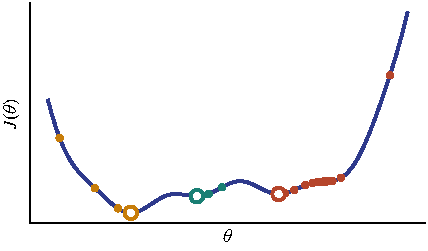
\includegraphics[width=0.46\linewidth]{figures/n7_nonconvex.pdf}
\caption{Gradient descent ($\eta = 0.02$, 200 steps) from $\theta_0 = -2.8$, $0$ and $2.9$ on a non-convex function
ends in three different local minima (open circles), at $\theta = -1.57$, $-0.43$ and $0.98$; only the first is the
global minimum.}
\label{fig:nonconvex}
\end{figure}

\needspace{8\baselineskip}
\section{Stochastic gradients}\label{sec:sgd}

\subsection{The gradient of a mean}

\paragraph{Derivation: the gradient of a mean is the mean of the gradients} Differentiation is linear: the
derivative of a sum is the sum of the derivatives and constants factor out. Applying this to each component
$\partial/\partial\theta_k$ of $J(\theta) = \frac1n\sum_i L_i(\theta)$, where $L_i(\theta) = L(f_\theta(\x_i), y_i)$,
\[
  \nabla J(\theta) = \nabla\Big(\frac1n \sum_{i=1}^n L_i(\theta)\Big) = \frac1n \sum_{i=1}^n \nabla L_i(\theta) \quad (+\,\lambda\nabla\Omega).
\]
\emph{Batch} gradient descent computes all $n$ terms before every update, which costs a full pass over the data per
step: for $n = 10^6$ images, one step means processing a million images. \emph{Mini-batch} gradient descent replaces the
mean over $\Dtrain$ by the mean over a random subset $B$ of $n' \ll n$ examples:
\[
  \gvec_B(\theta) = \frac{1}{n'} \sum_{i \in B} \nabla L_i(\theta), \qquad
  \theta \leftarrow \theta - \eta\, \gvec_B(\theta) .
\]
The case $n' = 1$ is \emph{stochastic} (online) gradient descent, SGD; $n' = n$ recovers the batch method.

\subsection{\texorpdfstring{Mini-batch gradients are unbiased and their noise falls like $1/n'$}{Mini-batch gradients are unbiased and their noise falls like 1/n'}}

Let $\bar{\gvec} = \nabla J(\theta) = \frac1n\sum_i \nabla L_i$ and let
$\Sigma = \frac1n\sum_i (\nabla L_i - \bar{\gvec})(\nabla L_i - \bar{\gvec})\T$ be the covariance of the per-example
gradients over the training set (both at the current $\theta$).

\paragraph{Derivation: unbiasedness} Draw an index $I$ uniformly from $\{1, \dots, n\}$. Then
$\E[\nabla L_I] = \sum_i \frac1n \nabla L_i = \bar{\gvec}$. A mini-batch of $n'$ draws $I_1, \dots, I_{n'}$ gives
$\gvec_B = \frac{1}{n'}\sum_k \nabla L_{I_k}$, and by linearity of expectation
\[
  \E[\gvec_B] = \frac{1}{n'}\sum_{k=1}^{n'} \E[\nabla L_{I_k}] = \bar{\gvec} .
\]
On average, the mini-batch gradient points exactly where the full gradient points. (The same holds for batches drawn
without replacement, since each example is then equally likely to be in $B$.)

\paragraph{Derivation: variance} Each draw $\nabla L_{I_k}$ is a uniformly chosen per-example gradient, so its
covariance is $\Sigma$ by definition. If the $n'$ draws are independent (with replacement), the covariance of a sum of
independent vectors is the sum of their covariances, and a constant factor $a$ multiplies a covariance by $a^2$, so
\[
  \Cov[\gvec_B] = \frac{1}{n'^2}\sum_{k=1}^{n'} \Cov[\nabla L_{I_k}] = \frac{1}{n'^2}\, n'\,\Sigma = \frac{\Sigma}{n'} .
\]
Each component's standard deviation falls like $1/\sqrt{n'}$: quadrupling the batch halves the noise, while it
quadruples the cost of a step. Without replacement the covariance is smaller by the factor $(n - n')/(n - 1)$, which
vanishes for $n' = n$, as it should.

\begin{worked}{a mini-batch gradient from a table of four examples}
Fit $f(x) = wx + b$ with $L_i = \frac12(wx_i + b - y_i)^2$. With residual $r_i = wx_i + b - y_i$ the chain rule gives
$\partial L_i/\partial w = r_i x_i$ and $\partial L_i/\partial b = r_i$. At $(w, b) = (1, 0)$:
\begin{center}\small
\begin{tabular}{@{}ccccccc@{}}
\toprule
$i$ & $x_i$ & $y_i$ & $f(x_i)$ & $r_i$ & $\partial L_i/\partial w = r_ix_i$ & $\partial L_i/\partial b = r_i$ \\
\midrule
1 & 1 & 2 & 1 & $-1$ & $-1$ & $-1$ \\
2 & 2 & 3 & 2 & $-1$ & $-2$ & $-1$ \\
3 & 3 & 5 & 3 & $-2$ & $-6$ & $-2$ \\
4 & 4 & 6 & 4 & $-2$ & $-8$ & $-2$ \\
\midrule
\multicolumn{5}{@{}l}{mean (full gradient)} & $-4.25$ & $-1.5$ \\
\bottomrule
\end{tabular}
\end{center}
Here $J = \frac14(0.5 + 0.5 + 2 + 2) = 1.25$. The mini-batch $B = \{1, 3\}$ gives
$\gvec_B = \frac12\big((-1, -1) + (-6, -2)\big) = (-3.5, -1.5)$: same signs, different size. The six possible batches
of two give
\[
  \begin{gathered}
  \{1,2\}: (-1.5, -1), \qquad \{1,3\}: (-3.5, -1.5), \qquad \{1,4\}: (-4.5, -1.5), \\
  \{2,3\}: (-4, -1.5), \qquad \{2,4\}: (-5, -1.5), \qquad \{3,4\}: (-7, -2),
  \end{gathered}
\]
whose average is $(-4.25, -1.5)$, exactly the full gradient: unbiasedness. The $w$-component of a single-example
gradient has variance $8.19$ over the four examples; for batches of two drawn with replacement it is $8.19/2 = 4.09$,
and for the six pairs above (without replacement) $4.09 \times (4 - 2)/(4 - 1) = 2.73$. One update with
$\eta = 0.05$ and $B = \{1, 3\}$ moves $(w, b)$ from $(1, 0)$ to $(1 + 0.175,\ 0 + 0.075) = (1.175, 0.075)$ and
lowers the full objective from $1.25$ to $0.544$. (The least-squares solution is $(1.4, 0.5)$; the stability limit from
the Hessian eigenvalue $8.35$ is $\eta < 0.24$.)
\end{worked}

\subsection{Epochs, shuffling and the noise floor}

In practice the data are shuffled once per \emph{epoch} (one pass over $\Dtrain$) and cut into consecutive
mini-batches (Algorithm~\ref{alg:sgd}). Every example is then used exactly once per epoch, and the shuffling prevents systematic
patterns: data sorted by class would push the parameters back and forth between classes for whole stretches of an epoch.

\begin{algorithm}[tb]
\caption{Mini-batch stochastic gradient descent with shuffling}\label{alg:sgd}
\begin{algorithmic}[1]
\Require training set $\{(\x_i, y_i)\}_{i=1}^n$; start $\theta_0$; batch size $n'$; schedule $\eta_t$; number of epochs $E$; clipping threshold $G$ (optional)
\Ensure parameters $\theta$
\Function{MiniBatchSGD}{$\theta_0$}
  \State $\theta \gets \theta_0$, \quad $t \gets 0$
  \For{epoch $= 1, \dots, E$}
    \State $\pi \gets$ random permutation of $\{1, \dots, n\}$ \Comment{$O(n)$}
    \For{$j = 0, n', 2n', \dots$ while $j < n$}
      \State $B \gets \{\pi_{j+1}, \dots, \pi_{\min(j + n', n)}\}$
      \State $\gvec \gets \frac{1}{|B|}\sum_{i \in B} \nabla_\theta L\big(f_\theta(\x_i), y_i\big)$ \Comment{$O(n'p)$, vectorised}
      \State optional clipping: \textbf{if} $\norm{\gvec} > G$ \textbf{then} $\gvec \gets G\,\gvec/\norm{\gvec}$ \Comment{$O(p)$; Section~\ref{sec:early}}
      \State $\theta \gets \theta - \eta_t\,\gvec$, \quad $t \gets t + 1$
    \EndFor
    \State optionally evaluate the validation loss (Section~\ref{sec:early})
  \EndFor
  \State \Return $\theta$
\EndFunction
\end{algorithmic}
\end{algorithm}

\begin{runtime}{mini-batch SGD}
\textbf{Per update:} $O(n'p)$; with $\lceil n/n'\rceil$ updates per epoch, one epoch costs $O(np)$, the same as
\emph{one} batch gradient step. \textbf{Total:} $O(Enp)$ for $E$ epochs. \textbf{Memory:} $O(p)$ plus per-batch
intermediate values ($\propto n'$); the data can be streamed from disk. \textbf{Hardware:} the $n'$ gradients are
computed together as matrix products, so on a GPU a batch of 256 costs far less than 256 times one example (for small
models, hardly more than one example).
\end{runtime}

Figure~\ref{fig:sgd} compares the three on logistic regression with $n = 2000$. After one epoch, batch gradient descent
has taken one step; mini-batch descent with $n' = 32$ has taken 63 and is already within $0.013$ of the optimal loss.
With a constant step, however, the stochastic methods do not converge: they fluctuate in a band whose width is set by
the gradient noise and the learning rate. The reason is visible in the derivation above: at the minimum the full
gradient vanishes, but the per-example gradients do not ($\Sigma \ne 0$), so each step still moves $\theta$ by about
$\eta$ times the noise. Pure SGD, the noisiest, ends further from the optimum than batch descent; mini-batches are
the compromise used in practice.

\begin{figure}[tbp]
\centering
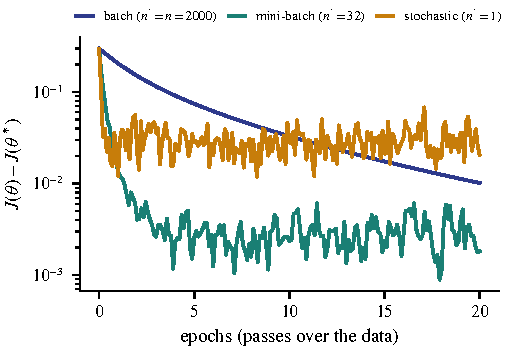
\includegraphics[width=0.52\linewidth]{figures/sgd.pdf}
\caption{Excess training loss of logistic regression ($d = 20$, $n = 2000$) against the number of passes over the data,
with constant learning rates. Mini-batch descent reaches $0.0018$ after 20 epochs; batch descent $0.010$; SGD
fluctuates between about $0.015$ and $0.07$ over the last epochs ($0.02$ at the end).}
\label{fig:sgd}
\end{figure}

Decreasing the learning rate removes the noise floor at the end of training. Robbins and Monro~\cite{robbins1951} gave
the classical conditions on the schedule,
\[
  \sum_{t} \eta_t = \infty, \qquad \sum_t \eta_t^2 < \infty :
\]
the steps must add up to an unlimited distance, so that any starting point can be left behind, while the accumulated
noise, whose variance grows like $\sum_t\eta_t^2$, stays finite. The $1/t$ schedule of Section~\ref{sec:schedules}
satisfies both; a constant step violates the second, and $\eta_t = 1/t^2$ violates the first.

\needspace{8\baselineskip}
\section{Beyond plain gradient descent}\label{sec:beyond}

\subsection{Momentum}\label{sec:momentum}

Accumulate a velocity and move with it:
\[
  \vvec_{t+1} = \beta\,\vvec_t - \eta\nabla J(\theta_t), \qquad \theta_{t+1} = \theta_t + \vvec_{t+1}, \qquad 0 \le \beta < 1,
\]
with $\vvec_0 = \vect{0}$; $\beta = 0$ is plain gradient descent. Unrolling the recursion,
$\vvec_{t+1} = -\eta\big(\gvec_t + \beta\gvec_{t-1} + \beta^2\gvec_{t-2} + \cdots\big)$: the step is an exponentially
weighted sum of past gradients. If the gradient keeps the same value $\gvec$, the velocity tends to
$-\eta\gvec\,(1 + \beta + \beta^2 + \cdots) = -\eta\gvec/(1 - \beta)$, an effective learning rate ten times larger for
$\beta = 0.9$. If it alternates in sign, $\pm\gvec$, the sum alternates, $1 - \beta + \beta^2 - \cdots = 1/(1 + \beta)$,
and its size tends to $\eta\norm{\gvec}/(1 + \beta)$: components of the gradient that keep their sign add up, those that
flip, as across a valley, cancel. As $\beta \to 1$ the friction vanishes: the effective step $\eta/(1 - \beta)$ grows
without bound, and the iterate overshoots and oscillates for a long time before it settles.

On a quadratic, Polyak's choice $\beta = \big((\sqrt\kappa - 1)/(\sqrt\kappa + 1)\big)^2$ and
$\eta = 4/(\sqrt{\lambda_{\max}} + \sqrt{\lambda_{\min}})^2$ improves the convergence factor per step from
$(\kappa - 1)/(\kappa + 1)$ to $(\sqrt\kappa - 1)/(\sqrt\kappa + 1)$~\cite{polyak1964}. The number of steps then grows
like $\sqrt\kappa$ instead of $\kappa$: for an error reduction of $10^{-6}$, 20 steps instead of 62 for $\kappa = 9$, 35
instead of 173 for $\kappa = 25$, and 691 instead of 69\,078 for $\kappa = 10^4$. In Figure~\ref{fig:gdpaths} momentum
reaches $J \approx 5 \times 10^{-10}$ in forty steps. Nesterov's accelerated gradient~\cite{nesterov1983}, a variant
that evaluates the gradient at the look-ahead point $\theta_t + \beta\vvec_t$ (one changed line in
Algorithm~\ref{alg:momentum}), provably needs only about $\sqrt\kappa\,\ln(1/\tau)$ iterations for all smooth, strongly
convex functions (Hessian eigenvalues bounded below by a positive constant everywhere), not only for quadratics.

\begin{algorithm}[H]
\caption{Gradient descent with momentum (heavy ball)}\label{alg:momentum}
\begin{algorithmic}[1]
\Require start $\theta_0$; learning rate $\eta$; momentum $\beta \in [0, 1)$ (typically $0.9$); number of steps $T$
\Ensure approximate minimiser $\theta$
\Function{Momentum}{$\theta_0$}
  \State $\theta \gets \theta_0$, \quad $\vvec \gets \vect{0}$
  \For{$t = 0, \dots, T - 1$}
    \State $\gvec \gets \nabla J(\theta)$ \Comment{or $\gvec_B$; Nesterov: $\gvec \gets \nabla J(\theta + \beta\vvec)$}
    \State $\vvec \gets \beta\vvec - \eta\gvec$ \Comment{$O(p)$}
    \State $\theta \gets \theta + \vvec$
  \EndFor
  \State \Return $\theta$
\EndFunction
\end{algorithmic}
\end{algorithm}

\begin{runtime}{momentum}
\textbf{Per iteration:} the gradient ($O(np)$ batch, $O(n'p)$ mini-batch) plus $O(p)$. \textbf{Memory:} one extra
vector $\vvec$. \textbf{Iterations:} about $\frac{\sqrt\kappa}{2}\ln(1/\tau)$ on a quadratic with tuned
$\eta, \beta$, against $\frac{\kappa}{2}\ln(1/\tau)$ without momentum --- for a negligible extra cost. Nesterov's
variant costs exactly the same: one gradient plus $O(p)$.
\end{runtime}

\begin{worked}{two momentum steps}
Return to $J = \frac12\theta\T A\theta$ with $A = \begin{pmatrix} 5 & 4 \\ 4 & 5\end{pmatrix}$, $\theta^{(0)} = (3, 1)$, and
take $\eta = 0.2$, $\beta = 0.25$.

\emph{Step 1.} $\gvec_0 = (19, 17)$, $\vvec_1 = 0.25 \cdot \vect{0} - 0.2\,(19, 17) = (-3.8, -3.4)$,
$\theta^{(1)} = (-0.8, -2.4)$, $J = 23.7$ --- the same as plain gradient descent, since the velocity starts at zero.

\emph{Step 2.} $\gvec_1 = A\theta^{(1)} = (-13.6, -15.2)$,
$\vvec_2 = 0.25\,(-3.8, -3.4) - 0.2\,(-13.6, -15.2) = (-0.95 + 2.72,\ -0.85 + 3.04) = (1.77, 2.19)$,
$\theta^{(2)} = (-0.8 + 1.77,\ -2.4 + 2.19) = (0.97, -0.21)$, $J = 1.65$.

Plain gradient descent with the same $\eta$ has $J = 15.2$ after two steps: the old velocity $(-3.8, -3.4)$ points
against the new descent step $-\eta\gvec_1 = (2.72, 3.04)$ along the steep direction $(1, 1)$, so the overshoot is
partly cancelled. Over more steps:
\begin{center}\small
\begin{tabular}{@{}lccccc@{}}
\toprule
method & $J(\theta^{(1)})$ & $J(\theta^{(2)})$ & $J(\theta^{(10)})$ & $J(\theta^{(20)})$ & error factor \\
\midrule
gradient descent, $\eta = 0.1$ & 1.17 & 0.660 & 0.122 & 0.0148 & 0.9 \\
gradient descent, $\eta = 0.2$ & 23.7 & 15.2 & 0.427 & 0.0049 & 0.8 \\
momentum, $\eta = 0.2$, $\beta = 0.25$ & 23.7 & 1.65 & 0.0010 & $5.0 \times 10^{-7}$ & 0.69 \\
momentum, $\eta = 0.25$, $\beta = 0.25$ & 56.8 & 36.2 & 0.0088 & $3.2 \times 10^{-8}$ & 0.5 \\
\bottomrule
\end{tabular}
\end{center}
The last row is Polyak's choice for $\kappa = 9$: $\beta = (2/4)^2 = 0.25$, $\eta = 4/(3 + 1)^2 = 0.25$, factor $0.5$.
Note that $\eta = 0.25$ alone diverges (previous worked example); the momentum term stabilises it. The last column
gives the asymptotic factor by which the \emph{error} shrinks per step, so $J$ shrinks by its square. For momentum it is
the largest $|r|$ among the roots of $r^2 - (1 + \beta - \eta\lambda_i)\,r + \beta = 0$ over both eigenvalues (the
eigenvalues of the $2 \times 2$ iteration matrix of Question~C3 with $a = \lambda_i$); for $\eta = 0.2$, $\beta = 0.25$ and $\lambda_i = 1$ the
roots are $0.685$ and $0.365$, for $\lambda_i = 9$ a complex pair of modulus $\sqrt\beta = 0.5$. Polyak's row starts with
a larger overshoot and a slower transient, and overtakes the momentum row with $\eta = 0.2$ only from step~15 on.
\end{worked}

\subsection{Newton's method}\label{sec:newton}

\paragraph{Derivation: the Newton step} Instead of the first-order model, minimise the second-order model of
\eqref{eq:taylor} around the current point,
\[
  m(\dvec) = J(\theta) + \gvec\T\dvec + \tfrac12\dvec\T H\dvec, \qquad \gvec = \nabla J(\theta),\ H = H(\theta).
\]
Its gradient with respect to $\dvec$ is $\gvec + H\dvec$ (Section~\ref{sec:lr}, with $H$ symmetric). Setting it to
zero gives $H\dvec = -\gvec$, so
\[
  \theta_{t+1} = \theta_t - H(\theta_t)^{-1}\,\nabla J(\theta_t) ,
\]
and the stationary point of $m$ is its minimum when $H$ is positive definite. In one dimension this is
$\theta \leftarrow \theta - J'(\theta)/J''(\theta)$: Newton's root-finding method applied to $J'$. Compared with
gradient descent, the Hessian rescales every eigen-direction by its own curvature, $1/\lambda_i$, which is the
per-direction step $\eta\lambda_i = 1$ that converged in one step in the one-dimensional example. Conditioning no
longer matters.

\begin{worked}{Newton steps}
\emph{On the quadratic} $J = \frac12\theta\T A\theta$ with $A = \begin{pmatrix} 5 & 4 \\ 4 & 5\end{pmatrix}$, the model
$m$ is $J$ itself. From $\theta^{(0)} = (3, 1)$: $A^{-1} = \frac19\begin{pmatrix} 5 & -4 \\ -4 & 5\end{pmatrix}$ and
$A^{-1}\gvec_0 = \frac19(5 \cdot 19 - 4 \cdot 17,\ -4 \cdot 19 + 5 \cdot 17) = \frac19(27, 9) = (3, 1)$, so
$\theta^{(1)} = (3, 1) - (3, 1) = (0, 0)$: the exact minimum in one step, whatever the condition number.

\emph{On the non-quadratic landscape} $J = \frac14\theta_1^4 - \theta_1\theta_2 + \frac12\theta_2^2$ from $(2, 1)$:
$\gvec = (7, -1)$ and $H = \begin{pmatrix} 12 & -1 \\ -1 & 1\end{pmatrix}$ with $\det H = 11$, so
$H^{-1} = \frac1{11}\begin{pmatrix} 1 & 1 \\ 1 & 12\end{pmatrix}$ and
$H^{-1}\gvec = \frac1{11}(7 - 1,\ 7 - 12) = (\frac6{11}, -\frac5{11})$. The new point is
$\theta^{(1)} = (2 - \frac6{11},\ 1 + \frac5{11}) = (\frac{16}{11}, \frac{16}{11}) = (1.4545, 1.4545)$. Repeating, the
iterates stay on the diagonal and approach the minimum $(1, 1)$:
\begin{center}\small
\begin{tabular}{@{}lcccccc@{}}
\toprule
step $t$ & 0 & 1 & 2 & 3 & 4 & 5 \\
\midrule
$\theta^{(t)}_1 - 1$ & $1$ & $0.455$ & $0.151$ & $0.0253$ & $9.1 \times 10^{-4}$ & $1.2 \times 10^{-6}$ \\
\bottomrule
\end{tabular}
\end{center}
Once close, the error is roughly squared at each step (the number of correct digits doubles): \emph{quadratic
convergence}. Gradient descent with $\eta = 0.1$ from the same start needs 86 steps to bring both coordinates
within $10^{-3}$ of the minimum and about 200 to match the accuracy Newton reaches in five (Figure~\ref{fig:quartic}). From $(0.3, 0.5)$, however, Newton's method jumps to $(-0.074, -0.074)$ and then converges
to the saddle $(0, 0)$, where $H$ is indefinite: it looks for stationary points, not specifically for minima.
\end{worked}

The remedies for this behaviour are standard~\cite{nocedal2006}: add $\mu I$ to $H$ until it is positive definite
(a \emph{Hessian modification}, the idea behind the Levenberg--Marquardt method for least squares), which makes
$\dvec$ a descent direction; take a \emph{damped} step $\alpha\dvec$ with $\alpha$ chosen by line search; or restrict
the step to a region where the quadratic model can be trusted (trust-region methods). Algorithm~\ref{alg:newton}
combines the first two. With it, the run from $(0.3, 0.5)$ uses $\mu = 0.512$ and $\alpha = \frac14$ in its first step
and reaches the minimum $(1, 1)$, to eight digits, in three steps instead of the saddle.

\begin{algorithm}[H]
\caption{Damped Newton's method with Hessian modification}\label{alg:newton}
\begin{algorithmic}[1]
\Require start $\theta_0$; gradient $\nabla J$ and Hessian $H(\theta)$; tolerance $\epsilon_g$; maximum $T$; Armijo constant $c \in (0, 1)$ (e.g.\ $10^{-4}$)
\Ensure approximate minimiser $\theta$
\Function{Newton}{$\theta_0$}
  \State $\theta \gets \theta_0$
  \For{$t = 0, \dots, T - 1$}
    \State $\gvec \gets \nabla J(\theta)$ \Comment{$O(np)$}
    \If{$\norm{\gvec} < \epsilon_g$} \Return $\theta$ \EndIf
    \State $H \gets H(\theta)$, \quad $\mu \gets 0$ \Comment{$O(np^2)$ to form, $O(p^2)$ memory}
    \While{the Cholesky factorisation of $H + \mu I$ fails} \Comment{$O(p^3)$ per attempt}
      \State $\mu \gets \max(2\mu, 10^{-3})$ \Comment{until $H + \mu I$ is positive definite}
    \EndWhile
    \State solve $(H + \mu I)\dvec = -\gvec$ with the factor \Comment{$O(p^2)$; never form $H^{-1}$}
    \State $\alpha \gets 1$ \Comment{$\gvec\T\dvec < 0$: a descent direction}
    \While{$J(\theta + \alpha\dvec) > J(\theta) + c\,\alpha\,\gvec\T\dvec$} $\alpha \gets \alpha/2$ \EndWhile
    \Statex \hfill\Comment{Armijo test of Section~\ref{sec:linesearch} with $\dvec$ in place of $-\gvec$}
    \State $\theta \gets \theta + \alpha\dvec$
  \EndFor
  \State \Return $\theta$
\EndFunction
\end{algorithmic}
\end{algorithm}

\begin{runtime}{Newton's method}
\textbf{Per iteration:} gradient $O(np)$; Hessian $O(np^2)$ (for logistic regression $H = \frac1n X\T S X$, with
$X$ the $n \times (d + 1)$ data matrix and $S$ a diagonal matrix of per-example weights, Note~9, Section~4: $O(nd^2)$); solving the $p \times p$ system $O(p^3)$. \textbf{Memory:} $O(p^2)$. \textbf{Iterations:}
typically 5 to 20. For $p$ up to a few thousand this is an excellent trade, and logistic regression is often trained
this way. In 32-bit floats the Hessian needs 4~TB for $p = 10^6$ and 40~PB for $p = 10^8$ (the parameters: 0.4~GB).
Mini-batches do not rescue it: a Hessian estimated from a mini-batch is noisy, and inverting it amplifies the noise
along its smallest eigenvalues, so steps can explode. Stochastic training therefore uses cheap diagonal rescalings
instead, such as Adam's division by $\sqrt{\hat{\vect{s}}}$ (Section~\ref{sec:adam}).
\end{runtime}

Between the two extremes lie methods that use curvature without storing $H$; we name them for orientation only,
their details are beyond this course~\cite{nocedal2006}. \emph{Quasi-Newton} methods such as L-BFGS approximate
$H^{-1}$ by a scaled identity corrected with $M$ rank-two updates built from the last $M$ (typically 5--20) differences
of gradients and parameters, at $O(Mp)$ extra time and memory per step. The \emph{conjugate gradient} method,
which minimises a quadratic in at most $p$ steps using only products of the Hessian with vectors, is simple enough to treat in full.

\subsection{Conjugate gradient}\label{sec:cg}

Take the quadratic $J(\theta) = \frac12\theta\T A\theta - \vect{b}\T\theta$ with $A$ symmetric positive definite (least
squares has this form, Note~8), whose minimiser solves $A\theta = \vect{b}$. The residual
$\vect{r} = \vect{b} - A\theta = -\nabla J$ is the steepest-descent direction. The conjugate gradient
method~\cite{hestenes1952} moves along directions $\vect{d}_t$ that start from the residual but are corrected by a
multiple of the previous direction so that they are \emph{$A$-conjugate}, $\vect{d}_s\T A\vect{d}_t = 0$ for $s \ne t$,
and along each one it takes the exact minimising step: setting $\frac{d}{d\alpha}J(\theta + \alpha\vect{d}) =
-\vect{r}\T\vect{d} + \alpha\,\vect{d}\T A\vect{d}$ to zero gives $\alpha = \vect{r}\T\vect{d}/\vect{d}\T A\vect{d}$, which
equals $\vect{r}\T\vect{r}/\vect{d}\T A\vect{d}$ for these directions. Conjugate directions do not undo each other's
progress, so in exact arithmetic the minimum is reached in at most $p$ steps; in practice the error falls by a factor
$\tau$ in about $\frac{\sqrt\kappa}{2}\ln(2/\tau)$ steps~\cite{nocedal2006}, the same $\sqrt\kappa$ as tuned momentum but
without having to know $\lambda_{\min}$ and $\lambda_{\max}$. For a non-quadratic $J$, \emph{nonlinear} conjugate
gradient (Fletcher--Reeves, Polak--Ribi\`ere) uses $-\nabla J$ for $\vect{r}$ and a line search for $\alpha$.

\begin{algorithm}[H]
\caption{Linear conjugate gradient for $A\theta = \vect{b}$}\label{alg:cg}
\begin{algorithmic}[1]
\Require symmetric positive definite $A$ (or a routine computing $A\vect{u}$); $\vect{b}$; start $\theta_0$; tolerance $\epsilon_g$
\Ensure minimiser $\theta$ of $\frac12\theta\T A\theta - \vect{b}\T\theta$
\Function{ConjugateGradient}{$\theta_0$}
  \State $\theta \gets \theta_0$, \quad $\vect{r} \gets \vect{b} - A\theta$, \quad $\vect{d} \gets \vect{r}$
  \For{$t = 0, \dots, p - 1$}
    \If{$\norm{\vect{r}} < \epsilon_g$} \Return $\theta$ \EndIf
    \State $\vect{u} \gets A\vect{d}$ \Comment{the only product with $A$}
    \State $\alpha \gets \vect{r}\T\vect{r}/\vect{d}\T\vect{u}$ \Comment{exact minimum along $\vect{d}$}
    \State $\theta \gets \theta + \alpha\vect{d}$, \quad $\vect{r}_{\text{new}} \gets \vect{r} - \alpha\vect{u}$ \Comment{$\vect{r}_{\text{new}} = \vect{b} - A\theta$}
    \State $\beta \gets \vect{r}_{\text{new}}\T\vect{r}_{\text{new}}/\vect{r}\T\vect{r}$, \quad $\vect{d} \gets \vect{r}_{\text{new}} + \beta\vect{d}$, \quad $\vect{r} \gets \vect{r}_{\text{new}}$ \Comment{$O(p)$}
  \EndFor
  \State \Return $\theta$
\EndFunction
\end{algorithmic}
\end{algorithm}

\begin{runtime}{conjugate gradient}
\textbf{Per iteration:} one product $A\vect{d}$ plus $O(p)$: $O(p^2)$ for a dense $A$, and $O(np)$ for least squares,
where $A\vect{d} = \frac1n X\T(X\vect{d})$ is computed with two matrix--vector products without ever forming $A$.
\textbf{Memory:} four vectors, $O(p)$, beyond the data. \textbf{Iterations:} at most $p$ in exact arithmetic, about
$\frac{\sqrt\kappa}{2}\ln(2/\tau)$ in practice. It needs exact gradients, so like line search it is a method for
deterministic, full-batch problems.
\end{runtime}

\begin{worked}{conjugate gradient on the running quadratic}
For $A = \begin{pmatrix} 5 & 4 \\ 4 & 5\end{pmatrix}$, $\vect{b} = \vect{0}$ and $\theta^{(0)} = (3, 1)$:
$\vect{r}_0 = \vect{d}_0 = (-19, -17)$, $\vect{u} = A\vect{d}_0 = (-163, -161)$, $\vect{r}_0\T\vect{r}_0 = 650$,
$\vect{d}_0\T\vect{u} = 5834$, so $\alpha_0 = 0.111$ and $\theta^{(1)} = (0.883, -0.894)$ with $J = 0.790$ (gradient
descent with $\eta = 0.1$: $1.17$). The new residual $\vect{r}_1 = (-0.839, 0.938)$ is orthogonal to $\vect{r}_0$;
$\beta_0 = 1.584/650 = 0.00244$, $\vect{d}_1 = (-0.886, 0.897)$ and $\alpha_1 = 0.997$ give $\theta^{(2)} = (0, 0)$
exactly. With $p = 2$, two steps suffice; Newton's method needs only one, but it must solve a linear system with $A$, whereas conjugate gradient only multiplies vectors by $A$.
\end{worked}

\subsection{Adaptive methods: Adam and AdamW}\label{sec:adam}

Adam~\cite{kingma2015} keeps exponential moving averages of the gradient and of its element-wise square,
\[
  \mvec_t = \beta_1\mvec_{t-1} + (1 - \beta_1)\,\gvec_t, \qquad
  \vect{s}_t = \beta_2\vect{s}_{t-1} + (1 - \beta_2)\,\gvec_t^2 ,
\]
with $\mvec_0 = \vect{s}_0 = \vect{0}$, and moves each parameter by its averaged gradient divided by the root mean
square of its recent gradients:
\[
  \theta_{t} = \theta_{t-1} - \eta\,\frac{\hat{\mvec}_t}{\sqrt{\hat{\vect{s}}_t} + \epsilon}, \qquad
  \hat{\mvec}_t = \frac{\mvec_t}{1 - \beta_1^t}, \quad \hat{\vect{s}}_t = \frac{\vect{s}_t}{1 - \beta_2^t},
\]
all operations element-wise; typical values are $\beta_1 = 0.9$, $\beta_2 = 0.999$, $\epsilon = 10^{-8}$.

\paragraph{Derivation: the bias correction} Unrolling the recursion from $\mvec_0 = \vect{0}$,
$\mvec_t = (1 - \beta_1)\sum_{j=1}^{t}\beta_1^{t-j}\gvec_j$. If all gradients were equal to $\gvec$, the geometric sum
would give $\mvec_t = (1 - \beta_1)\,\frac{1 - \beta_1^t}{1 - \beta_1}\,\gvec = (1 - \beta_1^t)\,\gvec$, which is too small at
the start because the average was initialised at zero. Dividing by $1 - \beta_1^t$ removes this bias; the same
argument applies to $\vect{s}_t$. After many steps $\beta^t \to 0$ and the correction disappears.

The ratio $\hat{\mvec}/\sqrt{\hat{\vect{s}}}$ is dimensionless and of order one in size: $\hat{\mvec}$ is an average of
recent gradients and $\sqrt{\hat{\vect{s}}}$ their root mean square, and the size of an average never exceeds the root
mean square (their squares differ by a variance, which is non-negative). With equal weights in the two averages the
ratio is at most $1$, with equality when the gradient keeps a constant sign and size; with $\beta_1 \ne \beta_2$ this
holds approximately. So the step of each parameter is typically of size $\eta$ (and bounded by a small multiple of
it), whatever the scale of its gradient. This compensates for very different gradient scales across the layers of a
network, the per-parameter analogue of standardising the features. The price: the step no longer shrinks as the
gradient shrinks, so near a minimum Adam keeps moving by about $\eta$ unless $\eta$ is decayed
(Section~\ref{sec:schedules}), and it stores two extra vectors.

\begin{worked}{Adam's first steps}
Let $J = \frac12(\theta_1^2 + 25\,\theta_2^2)$, so $\gvec = (\theta_1, 25\theta_2)$, start at $(2, 1)$ and use
$\eta = 0.1$, $\beta_1 = 0.9$, $\beta_2 = 0.999$ ($\epsilon$ negligible).

\emph{Step 1.} $\gvec_1 = (2, 25)$; $\mvec_1 = 0.1\,\gvec_1 = (0.2, 2.5)$; $\vect{s}_1 = 0.001\,\gvec_1^2 = (0.004, 0.625)$;
the corrections divide by $0.1$ and $0.001$, so $\hat{\mvec}_1 = (2, 25)$ and $\hat{\vect{s}}_1 = (4, 625)$. The step is
$0.1\,(2/2,\ 25/25) = (0.1, 0.1)$ and $\theta^{(1)} = (1.9, 0.9)$. The first Adam step is $\eta\,\operatorname{sign}(\gvec)$.

\emph{Step 2.} $\gvec_2 = (1.9, 22.5)$; $\mvec_2 = 0.9\,(0.2, 2.5) + 0.1\,(1.9, 22.5) = (0.37, 4.5)$;
$\vect{s}_2 = 0.999\,(0.004, 0.625) + 0.001\,(3.61, 506.25) = (0.007606, 1.1306)$. With $1 - 0.9^2 = 0.19$ and
$1 - 0.999^2 = 0.001999$: $\hat{\mvec}_2 = (1.947, 23.68)$, $\hat{\vect{s}}_2 = (3.805, 565.6)$,
$\sqrt{\hat{\vect{s}}_2} = (1.951, 23.78)$, and the step is $(0.0998, 0.0996)$, so $\theta^{(2)} = (1.800, 0.800)$.

Both coordinates move by almost exactly $\eta$, although their gradients differ by a factor of 12. Plain gradient
descent must keep $\eta < 2/25 = 0.08$ for stability; with $\eta = 0.07$ its first step moves the component $\theta_1$ by only $0.14$
and $\theta_2$ by $1.75$, overshooting to $(1.86, -0.75)$.
\end{worked}

\paragraph{Weight decay: Adam versus AdamW} Adding $\frac\lambda2\norm{\theta}^2$ to $J$ adds $\lambda\theta$ to the
gradient. In Adam this term is then divided by $\sqrt{\hat{\vect{s}}}$, so parameters with large gradients are barely
regularised. AdamW~\cite{loshchilov2019} instead \emph{decouples} the decay, subtracting $\eta_t\lambda\theta$ directly
in the update (line~\ref{line:decay} of Algorithm~\ref{alg:adam}), so every parameter shrinks at the same relative rate.
(This is the convention of common libraries such as PyTorch, where the decay is scaled by the learning rate; the original
paper scales $\lambda$ by the schedule multiplier only, so the same nominal $\lambda$ can mean different things.)
For plain gradient descent the two are identical; for adaptive methods they are not, and AdamW is the default
optimiser for transformers.

\begin{algorithm}[tb]
\caption{Adam and AdamW}\label{alg:adam}
\begin{algorithmic}[1]
\Require start $\theta_0$; learning rates $\eta_t$; $\beta_1, \beta_2 \in [0, 1)$; $\epsilon > 0$; weight decay $\lambda \ge 0$ ($\lambda = 0$: Adam); number of steps $T$
\Ensure parameters $\theta$
\Function{AdamW}{$\theta_0$}
  \State $\theta \gets \theta_0$, \quad $\mvec \gets \vect{0}$, \quad $\vect{s} \gets \vect{0}$
  \For{$t = 1, \dots, T$}
    \State $\gvec \gets \gvec_B(\theta)$ \Comment{mini-batch gradient, $O(n'p)$}
    \State $\mvec \gets \beta_1\mvec + (1 - \beta_1)\gvec$, \quad $\vect{s} \gets \beta_2\vect{s} + (1 - \beta_2)\,\gvec \odot \gvec$ \Comment{$\odot$: element-wise product}
    \State $\hat{\mvec} \gets \mvec/(1 - \beta_1^t)$, \quad $\hat{\vect{s}} \gets \vect{s}/(1 - \beta_2^t)$
    \State $\theta \gets \theta - \eta_t\big(\hat{\mvec}/(\sqrt{\hat{\vect{s}}} + \epsilon) + \lambda\,\theta\big)$ \label{line:decay} \Comment{element-wise; $\lambda\theta$: decoupled decay}
  \EndFor
  \State \Return $\theta$
\EndFunction
\end{algorithmic}
\end{algorithm}

\begin{runtime}{Adam and AdamW}
\textbf{Per iteration:} the mini-batch gradient, $O(n'p)$, plus $O(p)$ element-wise operations. \textbf{Memory:}
$\mvec$ and $\vect{s}$ double the model size; with parameters and gradient, about $4p$ numbers --- 1.6~GB for $p = 10^8$
in 32-bit floats, against 40~PB for a Hessian. \textbf{Prediction:} unchanged; $\mvec, \vect{s}$ are discarded.
\end{runtime}

\subsection{Where the gradients come from}\label{sec:autodiff}

Every method above needs $\nabla J$. The definition of the partial derivative suggests \emph{finite differences}: the
forward difference $\big(J(\theta + h\evec_k) - J(\theta)\big)/h$ has error $O(h)$, the central difference
\[
  \frac{\partial J}{\partial\theta_k}(\theta) \approx \frac{J(\theta + h\evec_k) - J(\theta - h\evec_k)}{2h}
\]
has error $O(h^2)$, because the second-order Taylor terms cancel: by \eqref{eq:taylor},
$J(\theta \pm h\evec_k) = J(\theta) \pm h\,\partial J/\partial\theta_k + \frac12h^2H_{kk} + O(h^3)$, so the difference is
$2h\,\partial J/\partial\theta_k + O(h^3)$. The step cannot be made arbitrarily small: rounding
errors in the difference of two nearly equal numbers grow like $1/h$; in double precision $h \approx 10^{-5}$ is a good
compromise for the central difference. For
$J = \frac14\theta_1^4 - \theta_1\theta_2 + \frac12\theta_2^2$ at $(2, 1)$, where the exact gradient is $(7, -1)$, the
forward differences give $(7.620, -0.950)$ for $h = 0.1$ and $(7.060, -0.995)$ for $h = 0.01$; the central differences
give $(7.020, -1.000)$ and $(7.0002, -1.0000)$: dividing $h$ by ten divides the forward error by ten and the
central error by a hundred.

\begin{algorithm}[tb]
\caption{Gradient by central differences}\label{alg:fd}
\begin{algorithmic}[1]
\Require function $J$; point $\theta \in \R^p$; step $h$
\Function{FiniteDifferenceGradient}{$\theta, h$}
  \For{$k = 1, \dots, p$}
    \State $g_k \gets \big(J(\theta + h\evec_k) - J(\theta - h\evec_k)\big)/(2h)$ \Comment{two evaluations of $J$}
  \EndFor
  \State \Return $\gvec = (g_1, \dots, g_p)$
\EndFunction
\end{algorithmic}
\end{algorithm}


\begin{runtime}{finite differences versus automatic differentiation}
\textbf{Finite differences:} $2p$ evaluations of $J$, each $O(np)$, so $O(np^2)$ per gradient; for $p = 10^6$ that is
two million passes over the data for a single step. \textbf{Reverse-mode automatic differentiation} (backpropagation)
computes the exact gradient at a cost of a small constant times one evaluation of $J$, $O(np)$, independently of
$p$~\cite{baydin2018}; its price is memory, since the intermediate values of the forward computation are stored for the
backward pass. Finite differences remain useful for \emph{gradient checking}: comparing a hand-coded or automatic
gradient with Algorithm~\ref{alg:fd} on a few random coordinates catches most bugs. How reverse mode achieves its
cost is the subject of the week~5 notes on neural networks.
\end{runtime}

\subsection{Constraints}\label{sec:constraints}

Parameters may have to satisfy constraints: a variance must be positive, a spin direction must have unit length, the
weights of a mixture must form a probability vector (non-negative, summing to one). One can reparameterise (write
$\sigma^2 = e^u$, or obtain the mixture weights from free parameters $u_k$ through the softmax
$w_k = e^{u_k}/\sum_j e^{u_j}$, which is positive and sums to one), use Lagrange multipliers, or project.
\emph{Projected gradient descent} (Algorithm~\ref{alg:pgd}) changes a single line of Algorithm~\ref{alg:gd}:
$\theta \gets \Pi(\theta - \eta\gvec)$, where $\Pi$ returns the nearest feasible point. For non-negativity $\Pi$ sets
negative components to zero; for a unit-length direction it divides by the norm.

\begin{algorithm}[tb]
\caption{Projected gradient descent}\label{alg:pgd}
\begin{algorithmic}[1]
\Require gradient $\nabla J$; projection $\Pi$ onto the feasible set; feasible start $\theta_0$; learning rate $\eta$; number of steps $T$
\Ensure feasible approximate minimiser $\theta$
\Function{ProjectedGD}{$\theta_0$}
  \State $\theta \gets \theta_0$
  \For{$t = 0, \dots, T - 1$}
    \State $\gvec \gets \nabla J(\theta)$ \Comment{$O(np)$}
    \State $\theta \gets \Pi(\theta - \eta\gvec)$ \Comment{gradient step, then back to the nearest feasible point}
  \EndFor
  \State \Return $\theta$
\EndFunction
\end{algorithmic}
\end{algorithm}

\begin{runtime}{projected gradient descent}
\textbf{Per iteration:} the gradient, $O(np)$, plus the projection: $O(p)$ for non-negativity, a box or a unit sphere,
$O(p\log p)$ for the probability simplex (by sorting). \textbf{Memory:} $O(p)$. \textbf{Iterations:} for a convex $J$
and a convex feasible set, of the same order as unconstrained gradient descent.
\end{runtime}

\begin{worked}{projected gradient descent with a non-negativity constraint}
Minimise $J = (\theta_1 + 1)^2 + (\theta_2 - 2)^2$ subject to $\theta_1, \theta_2 \ge 0$, with $\eta = 0.25$ from
$(1, 1)$; $\nabla J = (2(\theta_1 + 1),\ 2(\theta_2 - 2))$. Step 1: $(1, 1) - 0.25\,(4, -2) = (0, 1.5)$, already
feasible. Step 2: $(0, 1.5) - 0.25\,(2, -1) = (-0.5, 1.75)$, projected to $(0, 1.75)$. Step 3 gives $(0, 1.875)$.
The iterates approach $(0, 2)$ with $J = 1$, a point on the boundary; the unconstrained minimum $(-1, 2)$ is infeasible.
At the constrained minimum the gradient $(2, 0)$ does not vanish: it points into the feasible region, and $-\nabla J$
points out of it, so no feasible step can lower $J$.
\end{worked}

When the objective and all constraints are linear the problem is a \emph{linear programme}; a quadratic objective with
linear constraints is a \emph{quadratic programme}. Both have dedicated solvers (simplex and interior-point
methods~\cite{boyd2004}), and the support vector machine of Note~9, Section~5, is a quadratic programme.

\begin{physics}{optimisers as mechanics}
Gradient descent with small steps follows the \emph{gradient flow} $\dot\theta = -\nabla J(\theta)$: overdamped motion
of a particle in the potential $J$. The update \eqref{eq:gd} is the explicit Euler discretisation of this flow with
time step $\eta$, and the condition $\eta < 2/\lambda_{\max}$ is the familiar stability limit of explicit Euler for a
stiff system: the fastest mode sets the largest stable time step. Momentum restores inertia --- Polyak's ``heavy ball'',
$m\ddot\theta + \gamma\dot\theta = -\nabla J$, discretised --- so progress along the floor of a narrow valley builds up
speed, while oscillations across it are damped; with Polyak's tuning they still occur but shrink by a factor
$\sqrt\beta$ per step (Figure~\ref{fig:gdpaths}). The noise of mini-batch gradients acts like a temperature: SGD resembles Langevin dynamics, and adding
properly scaled Gaussian noise to the updates turns it into a sampler of the posterior distribution of the
parameters~\cite{welling2011}.
\end{physics}

\section{Stopping, monitoring and the cost of training}\label{sec:early}

\subsection{Early stopping}

The stopping rules of Algorithm~\ref{alg:gd} look at the training objective. For learning, what matters is the error
on new data, and that can start rising while the training loss still falls: the model begins to fit the noise of the
training set (Note~4, Section~5). \emph{Early stopping} monitors the loss on a validation set (Note~4, Section~4) after
every epoch, remembers the best parameters seen, and stops once the validation loss has not improved for a number of
epochs called the \emph{patience} (Algorithm~\ref{alg:early}). The number of steps then acts like a regularisation
hyperparameter: started from small weights, gradient descent on least squares stopped after few steps behaves much
like ridge regression (least squares plus a penalty $\lambda\norm{\vect{w}}^2$, Note~8). Along a low-curvature direction
$J$ barely changes, so the data determine the minimiser poorly there and noise in the data moves it a lot; by
Section~\ref{sec:lr}, gradient descent fits exactly these directions last (factor $1 - \eta\lambda_i$ close to one), so
stopping early leaves them near their small starting values, much as the ridge penalty does (see
also~\cite{goodfellow2016}, Section~7.8).

\begin{algorithm}[tb]
\caption{Early stopping with patience}\label{alg:early}
\begin{algorithmic}[1]
\Require initial $\theta$; one-epoch training routine (e.g.\ the inner loop of Algorithm~\ref{alg:sgd}); validation set $\Dvalid$ of $n_{\text{valid}}$ examples; patience $P$; maximum epochs $E$
\Function{EarlyStopping}{$\theta$}
  \State $\theta_{\text{best}} \gets \theta$, \quad $\ell_{\text{best}} \gets \infty$, \quad $k \gets 0$ \Comment{$k$: epochs without improvement}
  \For{epoch $= 1, \dots, E$}
    \State $\theta \gets$ \Call{TrainOneEpoch}{$\theta$} \Comment{$O(np)$}
    \State $\ell \gets$ validation loss of $f_\theta$ on $\Dvalid$ \Comment{$O(n_{\text{valid}}\,p)$}
    \If{$\ell < \ell_{\text{best}}$}
      \State $\ell_{\text{best}} \gets \ell$, \quad $\theta_{\text{best}} \gets \theta$, \quad $k \gets 0$ \Comment{copy: $O(p)$}
    \Else
      \State $k \gets k + 1$
      \If{$k = P$} \textbf{break} \EndIf
    \EndIf
  \EndFor
  \State \Return $\theta_{\text{best}}$
\EndFunction
\end{algorithmic}
\end{algorithm}


\begin{worked}{tracing early stopping}
Validation losses after epochs $1, \dots, 9$: $0.92, 0.61, 0.48, 0.44, 0.43, 0.45, 0.44, 0.47, 0.50$; $P = 3$. The best
improves up to epoch~5 ($0.43$). Epoch~6 sets the counter to 1; epoch~7 ($0.44$) beats epoch~6 but not the best, so
the counter becomes 2; epoch~8 makes it $3 = P$. Training stops and returns epoch~5's parameters; epoch~9 is never run.
\end{worked}

\begin{runtime}{early stopping}
\textbf{Overhead per epoch:} one validation pass, $O(n_{\text{valid}}\,p)$, and an $O(p)$ copy when the loss improves.
\textbf{Memory:} one extra copy of the parameters. It usually \emph{saves} time by ending training early. The
validation set used to stop cannot also give an unbiased error estimate; that is the job of the test set.
\end{runtime}

\paragraph{Gradient clipping} One unusual mini-batch can give a huge gradient and throw the parameters far away. \emph{Clipping}~\cite{pascanu2013} rescales the gradient when its norm exceeds a threshold $G$: if
$\norm{\gvec} > G$, replace $\gvec$ by $G\,\gvec/\norm{\gvec}$ (optional line of Algorithm~\ref{alg:sgd}). For example,
$\gvec = (6, 8)$ with $G = 5$ becomes $(3, 4)$. The direction is kept, only the length is limited; the cost is $O(p)$.

\begin{modern}{how a large language model is trained}
The recipe for GPT-3, typical of large models, uses many of the ideas above~\cite{brown2020}: Adam with $\beta_1 = 0.9$
and $\beta_2 = 0.95$, the gradient norm clipped at 1.0 to tame rare large steps, a linear warm-up over the first 375
million tokens followed by cosine decay of the learning rate to 10\% of its peak over 260 billion tokens
(Section~\ref{sec:schedules}), weight decay of 0.1, and mini-batches that grow to about 3.2 million tokens. No
second-order method, line search or validation-based early stopping is used at this scale. The objective is the next-token cross-entropy (Note~2, Section~2), and each
update is a mini-batch gradient step of Section~\ref{sec:sgd}, on $1.75 \times 10^{11}$ parameters. Stored as 32-bit
numbers, the parameters and the two Adam moment vectors alone would occupy $3 \times 700\ \text{GB} = 2.1$~TB, so the
optimiser state is spread over many accelerators; anything quadratic in $p$, such as a Hessian, is out of the question.
\end{modern}

\paragraph{Costs at a glance} Table~\ref{tab:costs} collects the running times of this note (prediction cost depends
only on the model).

\begin{table}[H]
\centering\small
\caption{Cost of the optimisation methods of this note: work per iteration, memory beyond the data, and typical number
of iterations ($\kappa$: condition number, $\tau$: target accuracy, $M$: L-BFGS history length).}
\label{tab:costs}
\begin{tabular}{@{}L{3.3cm}L{2.5cm}L{2.3cm}L{6.2cm}@{}}
\toprule
method & per iteration & memory & iterations and remarks \\
\midrule
batch gradient descent & $O(np)$ & $O(p)$ & $\sim\frac{\kappa}{2}\ln\frac1\tau$ on a quadratic (best fixed $\eta$) \\
\quad + line search & $O(np)$ per trial & $O(p)$ & no tuning of $\eta$; deterministic only \\
mini-batch SGD & $O(n'p)$ & $O(p)$ & $n/n'$ updates per epoch; noise floor if $\eta$ fixed \\
momentum & gradient $+ O(p)$ & $O(p)$ & $\sim\frac{\sqrt\kappa}{2}\ln\frac1\tau$ on a quadratic \\
Newton & $O(np^2 + p^3)$ & $O(p^2)$ & 5--20; quadratic convergence; small $p$ only \\
conjugate gradient & $O(np)$ (one $A\vect{d}$) & $O(p)$ & $\le p$; $\sim\frac{\sqrt\kappa}{2}\ln\frac2\tau$ on a quadratic \\
L-BFGS & $O(np + Mp)$ & $O(Mp)$ & medium $p$, deterministic problems \\
Adam / AdamW & $O(n'p)$ & $O(p)$ (${\approx}\,4p$) & default for deep networks \\
finite differences & $O(np^2)$ & $O(p)$ & checking only \\
reverse-mode AD & $O(np)$ & stored activations & how gradients are computed in practice \\
projected GD & $O(np)$ + projection & $O(p)$ & projection $O(p)$ to $O(p\log p)$ for simple sets \\
\bottomrule
\end{tabular}
\end{table}

\begin{keyidea}[Summary]
The gradient points uphill and vanishes at minima (stationarity); the Hessian describes curvature and classifies
stationary points. By Cauchy--Schwarz, $-\nabla J$ is the locally steepest direction, and gradient descent steps
along it with learning rate $\eta$. On a quadratic each eigen-direction is multiplied by $1 - \eta\lambda_i$ per step,
so stability needs $\eta < 2/\lambda_{\max}$ and the speed is limited by the condition number $\kappa$; standardised
features help. Convex objectives have a single basin; neural networks do not, but saddles rather than bad minima are the
usual obstacle. Mini-batch gradients are unbiased with variance $\propto 1/n'$: many cheap noisy steps, with a noise
floor that a decaying learning rate removes. Momentum cuts the dependence on $\kappa$ to $\sqrt\kappa$ at the cost of
one vector, and conjugate gradient achieves the same on quadratics without tuning; Newton's method removes it at
$O(p^2)$ memory and $O(p^3)$ time; Adam gives every parameter its own step size. Constraints are handled by
reparameterisation or projection, and discrete choices by search on validation data. Reverse-mode automatic differentiation supplies exact gradients at the cost of a few function evaluations, and
early stopping on validation data decides when to stop.
\end{keyidea}

\begin{questions}
\begin{conceptual}
\item Using the first-order Taylor expansion, explain why $-\nabla J(\theta)$ is the steepest descent direction. Why is
this only a \emph{local} statement?
\item True or false? Justify each answer in one sentence. (a) If $\nabla J(\theta) = \vect{0}$, then $\theta$ is a
minimum. (b) At a minimum of a differentiable function on $\R^p$ the gradient is zero. (c) The gradient is parallel to
the contour lines of $J$. (d) Every local minimum of a convex function is global.
\item What do the Hessian eigenvalues at a stationary point tell you? How does $\det H$ reveal a saddle when $p = 2$?
\item For batch gradient descent on a quadratic bowl, sketch (i) the path of $\theta$ across the valley and (ii) the
training loss against the iteration number when the learning rate is (a) much too small, (b) slightly below
$2/\lambda_{\max}$, (c) above $2/\lambda_{\max}$. Why does the loss still fall steadily in (b), even though $\theta$
jumps across the valley at every step?
\item Why does the condition number $\kappa = \lambda_{\max}/\lambda_{\min}$, and not the size of the eigenvalues,
determine how many steps gradient descent needs? How can standardising the features change $\kappa$?
\item For $J = \frac12\theta\T A\theta$ with $A = \begin{pmatrix} 5 & 4 \\ 4 & 5\end{pmatrix}$ (eigenvalue $9$ along
$(1, 1)$, eigenvalue $1$ along $(1, -1)$), gradient descent with $\eta = 0.2$ gives a larger $J$ than with
$\eta = 0.1$ after three steps but a much smaller one after forty. Explain why, using the per-direction factors
$1 - \eta\lambda_i$.
\item What does a learning-rate schedule do that a fixed learning rate cannot? Why do large models start with a
warm-up, and why does the learning rate decrease towards the end of training?
\item What does the Armijo condition of backtracking line search check, and why is line search common with full
gradients but rare with mini-batch gradients?
\item Give one convex and one non-convex objective mentioned in this note (the landscape of Figure~\ref{fig:quartic}
counts). Why is convexity useful, and why are
saddle points, rather than poor local minima, the usual obstacle in high-dimensional non-convex problems?
\item Compare batch, mini-batch and stochastic gradient descent: cost and noise of one update, updates per epoch,
use of parallel hardware.
\item The mini-batch gradient is unbiased. Why, then, does SGD with a constant learning rate not converge to the
minimiser? What is the role of each Robbins--Monro condition?
\item Doubling the batch size doubles the cost of a step. By what factor does the standard deviation of the gradient
estimate fall (batches drawn with replacement)? Why is the data set shuffled at the start of every epoch?
\item Explain with a heavy ball in a narrow valley why momentum helps. What happens for $\beta = 0$, and for $\beta$
very close to $1$?
\item Newton's method minimises any quadratic in one step. Give three reasons why it is not used to train a network
with $10^8$ parameters, and explain why it can converge to a saddle point.
\item Why does the first step of Adam move every parameter by about $\eta$, whatever the size of its gradient? Give one
advantage and one drawback of this behaviour.
\item What does AdamW change about weight decay compared with adding $\frac\lambda2\norm{\theta}^2$ to the loss in
Adam, and why does the difference matter only for adaptive methods?
\item Why are gradients of large models computed by automatic differentiation and not by finite differences? What are
finite differences still used for?
\item Why can stopping before the training loss reaches its minimum improve the test error? Which data set decides
when to stop, and why not the test set? What does the patience $P$ trade off?
\item What does gradient clipping change in an update, and what does it keep? Why is it useful with mini-batch
gradients?
\item Why can gradient descent not choose the number of neighbours $k$ of $k$-nearest neighbours, or minimise the 0--1
error of a classifier directly? What is done instead in each case?
\item Conjugate gradient and tuned momentum both need a number of steps proportional to $\sqrt\kappa$ on a quadratic.
What does conjugate gradient not need to know in advance, and why is it rarely used with mini-batch gradients?
\item In projected gradient descent, why does the gradient not have to vanish at the constrained minimum? Give one constraint
whose projection is cheap and one way to avoid the constraint by reparameterisation.
\end{conceptual}

\begin{calculations}
\item Let $J(\theta_1, \theta_2) = \theta_1^2 + \theta_1\theta_2 + \theta_2^2 - 3\theta_1$. (a) Compute $\nabla J$ and
the Hessian. (b) Find the stationary point and classify it. (c) Find the eigenvalues of $H$, the condition number and
the largest stable learning rate. (d) Perform one gradient-descent step from $(0, 0)$ with $\eta = 0.25$.
\item For $J(\theta) = 2(\theta - 1)^2$, write the gradient-descent update in the form
$\theta_{t+1} - 1 = a\,(\theta_t - 1)$. Starting from $\theta_0 = 0$, compute three steps for $\eta = 0.1$, $0.4$ and
$0.6$ and describe each behaviour. Which $\eta$ reaches the minimum in one step, and what is the stability limit?
\item Find the stationary points of $J(\theta_1, \theta_2) = \theta_1^2 - \theta_2^2 + \frac12\theta_2^4$ and classify
them with the Hessian. Starting at $(1, 0)$, where does gradient descent with a small step go? And starting at
$(1, 10^{-6})$? Explain the difference.
\item For $J = \frac12(\theta_1^2 + 25\,\theta_2^2)$ (Figure~\ref{fig:gdpaths}), substitute $\theta_2 = u/5$. Give the
condition numbers and largest stable learning rates before and after, and relate this to standardising features.
\item Fit $f(x) = wx$ (no intercept) with the loss $L_i = \frac12(wx_i - y_i)^2$ to the four examples
$(x, y) = (1, 2), (2, 3), (-1, -1), (3, 4)$. At $w = 0$ compute the four per-example gradients, the full gradient,
and the mini-batch gradients for $B = \{1, 2\}$ and $B = \{3, 4\}$. Check that the average of these two mini-batch
gradients equals the full gradient (the two batches split the data into equal halves, so this is the unbiasedness
of Section~\ref{sec:sgd} in miniature), and perform one SGD step with $B = \{1, 2\}$ and $\eta = 0.1$.
\item On $J(\theta) = (\theta - 3)^2$ from $\theta_0 = 0$, perform two steps of momentum with $\eta = 0.1$ and
$\beta = 0.5$ ($v_0 = 0$). Compare $\theta_2$ with two steps of plain gradient descent with the same $\eta$.
\item For $J(\theta) = e^\theta - 2\theta$, compute $J'$ and $J''$ and the minimiser. Perform two Newton steps from
$\theta_0 = 0$ and compare with two gradient-descent steps with $\eta = 0.5$ from the same start. Explain why gradient
descent does so well here (hint: compare $\eta$ with $1/J''(\theta^*)$). You may use $e^{0.5} = 1.649$.
\item (a) Compute the first Adam step ($\beta_1 = 0.9$, $\beta_2 = 0.999$, $\eta = 0.01$, $\epsilon$ negligible) for
the gradient $\gvec_1 = (0.01, -40)$ and explain the result. (b) A model has $p = 10^8$ parameters stored as 32-bit
floats. How much memory does its Hessian need? Compare with the memory for the parameters and the two moment
vectors of Adam (not counting the gradient).
\item (a) With $\eta_{\max} = 0.2$, compute the $1/t$ decay $\eta_t = \eta_{\max}t_0/(t_0 + t)$ with $t_0 = 50$ at
$t = 50$ and $t = 150$, and the warm-up-plus-cosine schedule $\eta_t = \eta_{\max}(t + 1)/W$ for $t < W$,
$\eta_t = \frac12\eta_{\max}\big(1 + \cos(\pi(t - W)/(T - W))\big)$ for $W \le t \le T$, with $W = 10$ and $T = 110$, at
$t = 0$, $4$, $60$ and $110$. (b) Early stopping with patience $P$ stops once the validation loss has not improved on
its best value for $P$ consecutive epochs, and returns the best parameters. The validation losses after epochs
$1, \dots, 8$ are $0.80$, $0.55$, $0.47$, $0.49$, $0.45$, $0.46$, $0.48$, $0.44$. With $P = 2$, after which epoch does
training stop, and which epoch's parameters are returned? Would $P = 3$ have changed the answer?
\end{calculations}

\begin{derivations}
\item Let $J(\theta) = \frac12\theta\T A\theta - \vect{b}\T\theta$ with $A$ symmetric positive definite. Derive
$\nabla J$, $H$ and $\theta^*$. Show that the error of gradient descent obeys $\errv_{t+1} = (I - \eta A)\errv_t$,
that $\eta = 2/(\lambda_{\max} + \lambda_{\min})$ reduces the error norm by at least $(\kappa - 1)/(\kappa + 1)$ per
step, and that Newton's method converges in one step from any start.
\item Show that the mini-batch gradient is unbiased and that its covariance is $\frac{1}{n'}$ times that of a
single-example gradient when the batch is drawn with replacement. Without replacement, show that the variance is
multiplied by $(n - n')/(n - 1)$ instead (hint: covariance of two different draws).
\item Apply momentum to $J(\theta) = \frac12 a\theta^2$ with curvature $a > 0$. Show that $(\theta_{t+1}, \theta_t)$ is
obtained from $(\theta_t, \theta_{t-1})$ by a $2 \times 2$ matrix, and that for $\beta = 0$ the convergence factor is
$|1 - \eta a|$. Show that a constant gradient $g$ leads to the limiting velocity $-\eta g/(1 - \beta)$.
\item Starting from the chord definition of convexity, derive the tangent-plane inequality
$J(\vect{b}) \ge J(\vect{a}) + \nabla J(\vect{a})\T(\vect{b} - \vect{a})$ and conclude that every stationary point of a
convex function is a global minimum. Show that the mean of convex losses plus $\lambda\norm{\theta}^2$ ($\lambda \ge 0$)
is convex.
\item For a one-dimensional $J$ with $J'(\theta^*) = 0$ and $J''(\theta^*) > 0$, expand $J'$ and $J''$ around $\theta^*$
to show that the Newton error $\Delta_t = \theta_t - \theta^*$ satisfies
$\Delta_{t+1} = \frac{J'''(\theta^*)}{2J''(\theta^*)}\,\Delta_t^2 + O(\Delta_t^3)$. Check the prediction numerically on
$J(\theta) = e^\theta - 2\theta$.
\end{derivations}

\begin{programming}
\item Implement batch, mini-batch and stochastic gradient descent for logistic regression and reproduce
Figure~\ref{fig:sgd}. Then give SGD the schedule $\eta_t = \eta_0/(1 + t/t_0)$ and report the excess loss after 20 epochs.
\item Implement gradient descent ($\eta = 0.1$), momentum ($\eta = 0.1$, $\beta = 0.5$), Newton's method (undamped) and
Adam ($\eta = 0.1$, $\beta_1 = 0.9$, $\beta_2 = 0.999$) for $J = \frac14\theta_1^4 - \theta_1\theta_2 + \frac12\theta_2^2$
(Figure~\ref{fig:quartic}). Count the iterations each needs to reach $\norm{\nabla J} < 10^{-8}$ from $(2, 1)$. Map the
starting points in $[-2, 2]^2$ from which undamped Newton converges to the saddle, and check that
Algorithm~\ref{alg:newton} avoids it.
\item Write a gradient checker (Algorithm~\ref{alg:fd}) for the logistic-regression loss. Plot the error of forward
and central differences against $h \in [10^{-12}, 10^{-1}]$ on log--log axes and explain the curves.
\end{programming}
\end{questions}

\paragraph{Further reading} Goodfellow, Bengio and Courville~\cite{goodfellow2016}, chapters~4 and~8; Bottou, Curtis
and Nocedal~\cite{bottou2018}; Nocedal and Wright~\cite{nocedal2006}; Boyd and Vandenberghe~\cite{boyd2004}.

\begin{thebibliography}{99}\small
\bibitem{armijo1966} L.~Armijo, Minimization of functions having Lipschitz continuous first partial derivatives, \emph{Pacific J.\ Math.}\ 16(1), 1--3 (1966).
\bibitem{baydin2018} A.~G. Baydin, B.~A. Pearlmutter, A.~A. Radul and J.~M. Siskind, Automatic differentiation in machine learning: a survey, \emph{J.\ Mach.\ Learn.\ Res.}\ 18(153), 1--43 (2018).
\bibitem{bottou2018} L.~Bottou, F.~E. Curtis and J.~Nocedal, Optimization methods for large-scale machine learning, \emph{SIAM Rev.}\ 60(2), 223--311 (2018).
\bibitem{boyd2004} S.~Boyd and L.~Vandenberghe, \emph{Convex Optimization}, Cambridge University Press (2004).
\bibitem{brown2020} T.~Brown \emph{et al.}, Language models are few-shot learners, \emph{NeurIPS} (2020).
\bibitem{dauphin2014} Y.~N. Dauphin \emph{et al.}, Identifying and attacking the saddle point problem in high-dimensional non-convex optimization, \emph{NeurIPS} (2014).
\bibitem{goodfellow2016} I.~Goodfellow, Y.~Bengio and A.~Courville, \emph{Deep Learning}, MIT Press (2016).
\bibitem{hestenes1952} M.~R. Hestenes and E.~Stiefel, Methods of conjugate gradients for solving linear systems, \emph{J.\ Res.\ Natl.\ Bur.\ Stand.}\ 49(6), 409--436 (1952).
\bibitem{kingma2015} D.~P. Kingma and J.~Ba, Adam: a method for stochastic optimization, \emph{ICLR} (2015).
\bibitem{loshchilov2017} I.~Loshchilov and F.~Hutter, SGDR: stochastic gradient descent with warm restarts, \emph{ICLR} (2017).
\bibitem{loshchilov2019} I.~Loshchilov and F.~Hutter, Decoupled weight decay regularization, \emph{ICLR} (2019).
\bibitem{nesterov1983} Yu.~E. Nesterov, A method for solving the convex programming problem with convergence rate $O(1/k^2)$, \emph{Soviet Math.\ Dokl.}\ 27, 372--376 (1983).
\bibitem{nocedal2006} J.~Nocedal and S.~J. Wright, \emph{Numerical Optimization}, 2nd ed., Springer (2006).
\bibitem{pascanu2013} R.~Pascanu, T.~Mikolov and Y.~Bengio, On the difficulty of training recurrent neural networks, \emph{ICML} (2013).
\bibitem{polyak1964} B.~T. Polyak, Some methods of speeding up the convergence of iteration methods, \emph{USSR Comput.\ Math.\ Math.\ Phys.}\ 4(5), 1--17 (1964).
\bibitem{robbins1951} H.~Robbins and S.~Monro, A stochastic approximation method, \emph{Ann.\ Math.\ Statist.}\ 22(3), 400--407 (1951).
\bibitem{welling2011} M.~Welling and Y.~W. Teh, Bayesian learning via stochastic gradient Langevin dynamics, \emph{ICML} (2011).
\end{thebibliography}

\SourceNote
\end{document}
